\documentclass[10pt]{article}
\usepackage[utf8]{inputenc}
\usepackage[T1]{fontenc}
\usepackage{glossaries}
\usepackage[acronym]{glossaries-extra}
\makeglossaries
\usepackage{nomencl}
\makenomenclature
\usepackage[french]{babel}
\usepackage{color}
\usepackage{fancyhdr}
\usepackage{graphicx}
\usepackage{hyperref}
\usepackage{subcaption}
\usepackage{float}
\usepackage{svg}
\usepackage{wrapfig}
\usepackage{adjmulticol}
\usepackage{titlesec}
\usepackage{geometry}
\usepackage{longtable}
\usepackage{array}
\usepackage{booktabs}
\usepackage{listingsutf8}
\usepackage{xcolor}
\usepackage{caption}
\usepackage{inconsolata} % police typewriter plus élégante
\usepackage{amsmath}
\usepackage{amssymb}
\usepackage{amsfonts}

\definecolor{codebg}{rgb}{0.97,0.97,0.97}
\definecolor{keywordcolor}{rgb}{0.2,0.2,0.6}
\definecolor{commentcolor}{rgb}{0.3,0.5,0.3}
\definecolor{stringcolor}{rgb}{0.5,0.2,0.2}


\setabbreviationstyle{long-short}

\newglossaryentry{openGL}
{
    name=openGL,
    description={Branche libre de la librairie graphique GL développée par
    Silicon Graphics en 1992 et reprise par le groupe Khronos à partir de
    2006}
}

\newglossaryentry{GLSL}
{
    name=GLSL,
    description={OpenGL Shading Language (GLSL) est un langage de
    programmation de shaders de haut niveau dont la syntaxe est fondée sur
    le langage C.}
}

\newglossaryentry{SDL2}
{
    name=SDL2,
    description={Simple DirectMedia Layer 2 (SDL2) est la deuxième version de
    SDL, une librairie graphique développée par Sam Lantinga ; acclamée pour
    sa portabilité et son accessibilité}
}

\newglossaryentry{vertex shader}
{
    name=vertex shader,
    description={Le \gls{vertex} shader est responsable du traitement des
    primitives (triangles, lignes, points) lors de la pipeline graphique}
}

\newglossaryentry{vertex}
{
    name=vertex,
    description={Un vertex est un point dans l'espace 3D qui définit la
    position d'un sommet d'une primitive (triangle, ligne, point) dans la
    pipeline graphique}
}

\newglossaryentry{fragment shader}
{
    name=fragment shader,
    description={Le fragment shader est responsable du traitement des
    fragments lors de la pipeline graphique}
}

\newglossaryentry{fragment}
{
    name=fragment,
    description={Un fragment est un composant graphique composé de peu de
    pixels qui constitue une primitive en informatique graphique}
}

\newglossaryentry{shader}
{
    name=shader,
    description={Un shader est un programme graphique compilé en microcode
    graphique sur le \gls{gpu}}
}

\newglossaryentry{rasteriser}
{
    name=rasteriser,
    description={(Informatique) Convertir des données numériques en points
    permettant leur impression ou leur affichage. \cite{lalanguefrancaise}}
}

\newglossaryentry{GBuffer}
{
    name=G-Buffer,
    description={Le GBuffer est un tampon de rendu utilisé dans le rendu
    différé pour stocker les informations de la scène, telles que la couleur,
    les normales et la profondeur}
}

\newglossaryentry{shadow mapping}
{
    name=shadow mapping,
    description={Le shadow mapping est une technique de rendu d'ombres
    utilisée dans le rendu différé. Elle consiste à créer une carte d'ombres
    (shadow map) qui stocke les informations de profondeur de la scène
    depuis la perspective de la source lumineuse. Lors du rendu, on
    compare la profondeur d'un fragment avec la profondeur stockée dans la
    shadow map pour déterminer s'il est dans l'ombre ou non}
}

\newglossaryentry{ssr}
{
    name=SSR,
    description={Le SSR (Screen Space Reflection) est une technique de rendu
    utilisée pour créer des réflexions réalistes en utilisant les
    informations de la scène stockées dans le \gls{GBuffer}. Elle permet de
    simuler des réflexions sur des surfaces réfléchissantes en se basant
    sur les pixels visibles à l'écran},
    text={SSR},
    first={SSR (Screen Space Reflection)}
}

\newglossaryentry{ssao}
{
    name=SSAO,
    description={L'SSAO (Screen Space Ambient Occlusion) est une technique de
    rendu utilisée pour simuler l'occlusion ambiante dans les scènes 3D. Elle
    permet de créer des ombres douces et réalistes en tenant compte de la
    géométrie de la scène et de la position des lumières},
    text={SSAO},
    first={SSAO (Screen Space Ambient Occlusion)}
}
\newglossaryentry{bloom}
{
    name=bloom,
    description={Le bloom est une technique de post-traitement utilisée pour
    simuler l'effet de diffusion de la lumière sur les surfaces brillantes.
    Elle crée un halo lumineux autour des objets lumineux pour améliorer le
    réalisme de la scène}
}
\newglossaryentry{smaa}
{
    name=SMAA,
    description={Le SMAA (Subpixel Morphological Anti-Aliasing) est une
    technique d'anti-aliasing utilisée pour réduire les artefacts de
    crénelage (souvent appelé \emph{effet escalier}) dans les images 3D. Elle combine plusieurs techniques
    d'anti-aliasing pour obtenir un rendu plus lisse et réaliste},
    text={SMAA},
    first={SMAA (Subpixel Morphological Anti-Aliasing)}
}

\newacronym{gpu}{GPU}{processeur graphique}
\hypersetup{
    colorlinks,
    citecolor=black,
    filecolor=black,
    linkcolor=black,
    urlcolor=black
}


\begin{document}

\lstdefinestyle{class_c}{
    backgroundcolor=\color{codebg},
    basicstyle=\ttfamily\small,
    keywordstyle=\color{keywordcolor}\bfseries,
    commentstyle=\color{commentcolor}\itshape,
    stringstyle=\color{stringcolor},
    frame=single,
    rulecolor=\color{gray},
    numbers=left,
    numberstyle=\tiny\color{gray},
    numbersep=5pt,
    tabsize=4,
    breaklines=true,
    captionpos=b,
    inputencoding=utf8/latin1,
    extendedchars=true,
    language=C++ % ou "C" selon besoin
}

\titleformat{\paragraph}
  {\normalfont\normalsize\bfseries} % Style (bold)
  {\theparagraph} % Numbering
  {1em} % Spacing between number and title
  {} % Format
  [\vspace{0.5em}] % Adds a vertical space after paragraph title
  \renewcommand{\theparagraph}{\thesubsubsection.\arabic{paragraph}}
  \setcounter{secnumdepth}{4} % Allows deeper numbering

\title{


    \begin{minipage}[t]{0.4\textwidth}
        \vspace{-2cm}
        
\includegraphics[width=\linewidth]{images/universite_logo.jpg}
    \end{minipage}
    \hfill
    \begin{minipage}[t]{0.4\textwidth}
        \vspace{-2cm}
        
\includegraphics[width=\linewidth]{images/ic2_logo.png}
    \end{minipage}
    
    \begin{center}
        \textbf{\textcolor{blue}{Le Mans Université}} \\ 
        Licence Informatique - \textit{2\up{e} année} \\ 
        Module 174UP02 Rapport de Projet \\
        \textbf{Chapper's Fallout}
    \end{center}
}

\author{
    Lucien Defosse, Ekrem Ayyildiz, Mehdi Ouaïl, Loup Picault
}

\date{\today}


\maketitle

\newpage
\tableofcontents
\newpage
    \textbf{Résumé}\\
    Ce projet consiste à développer un jeu vidéo d’horreur en 3D en langage C,
    se déroulant dans l’institut Claude Chappe. Le joueur doit y résoudre des
    mini-jeux tout en échappant à un monstre qui le poursuit. Le jeu repose sur
    un moteur 3D original, entièrement conçu par notre équipe, sans recourir à un
    moteur existant, et intègre modélisation 3D, gameplay et éléments sonores.
    Le projet s’inscrit dans le cadre de la formation de L2 Informatique de
    l’Université du Mans (année universitaire 2024–2025).\\\\
\section{Introduction}
Ce document présente le projet du jeu Chapper's Fallout réalisé dans le cadre de
la formation de L2 informatique de l’université du Mans pendant la période de
janvier à avril 2025 (mais développé en avance depuis septembre 2024). Ce projet
a été développé en langage C avec la librairie SDL.\\

Dans ce jeu, le joueur peut se déplacer dans l’institut Claude Chappe, avec pour
objectif de résoudre tous les mini-jeux 2D disponibles sur les PC disséminés dans
différents endroits de la zone. Il doit réussir cela tout en survivant au monstre
Chapper, qui le poursuit par moments, et en surmontant des parcours semés de trous
et de plateformes.\\

Le joueur possède un saut pour l’aider dans ces parcours, ainsi qu’une lampe torche
pour éclairer son chemin. Un tutoriel introduit les principes du jeu et les contrôles
permettant les déplacements, l’utilisation de la lampe et du saut avant que la
partie principale ne commence.\\

Nous présenterons dans une première partie notre jeu, ses scénarios d’utilisation
et ses principales fonctionnalités, puis dans une deuxième partie la gestion du
projet. Ensuite, dans une troisième partie, nous détaillerons les éléments principaux
de conception (algorithmes, structures de données, etc.). Nous exposerons par la
suite l’architecture de notre application (structuration du code en fichiers) avant
de montrer les principaux résultats obtenus. Enfin, nous conclurons sur les points
forts et les limites de notre travail, les écarts entre la planification
prévisionnelle et le déroulement réel du projet, ainsi que les leçons tirées de
cette expérience.\\

En annexe, nous présenterons un exemple de débogage et des tests (jeux d’essai
et cas de test d’un exemple au moins — le fichier .c étant disponible dans le
dépôt Git dans un répertoire dédié "test").
\newpage

\newpage
\section{Conception}

\subsection{Cahier des charges}

\textbf{- Contexte et objectifs du projet :}\\

Ce projet, réalisé dans le cadre de la L2 Informatique à l’Université du Mans, consiste à concevoir un jeu vidéo en langage C. Nous avons choisi de créer un jeu d’horreur en 3D prenant place dans l’institut Claude Chappe où le joueur explore un bâtiment, parfois poursuivi par un monstre, tout en résolvant des mini-jeux (voir détails dans l'introduction \ref{sec:intro}).\\

\textbf{- Contraintes techniques :}\\\\
- Langage imposé : C (exclusivement ou presque)  
- Aucune utilisation de moteur de jeu existant (Unity, Unreal…)  
- Bibliothèques autorisées : SDL / OpenGL  
- Durée du projet : janvier à avril 2025 (avec un travail amorcé dès septembre 2024)\\

\textbf{- Fonctionnalités prévues :}\\\\
- Déplacement en 3D dans une reproduction fidèle du bâtiment  
- Monstre poursuivant le joueur à certains moments  
- Mini-jeux en 2D intégrés dans des PC interactifs  
- Mécaniques de plateforme (saut, trous, obstacles)  
- Lampe torche pour éclairer l’environnement  
- Tutoriel expliquant les commandes\\

\textbf{- Architecture générale :}\\\\
Pour cela, nous développons notre propre moteur 3D, \textit{RaptiquaX}, en C avec SDL. L’institut est modélisé en 3D sur Blender, puis intégré au moteur. Un éditeur de niveau nous permet de placer objets, collisions et éléments interactifs. Les mini-jeux sont codés séparément puis intégrés au jeu.\\

\textbf{- Répartition des rôles :}\\\\
- \textbf{Lucien} : modélisation 3D du bâtiment/objets, design sonore\\ 
- \textbf{Loup} : moteur 3D, éditeur de niveau, mécaniques principales\\  
- \textbf{Ekrem} : conception et développement des mini-jeux  \\
- \textbf{Mehdi} : placement des collisions et éléments de jeu via l’éditeur\\

\newpage
\subsection{Fonctionnalités}
\newpage
\section{Organisation du projet}
    \subsection{Planning prévisionnel}
    \subsection{Répartition des tâches}
\newpage
\section{Développement}
\subsection{Création du moteur de jeu 3D}
    Pour composer les éléments du jeu et assurer une bonne qualité
    graphique et technique, le choix d'assembler le \emph{moteur de jeu 3D}
    \og \emph{RaptiquaX} \fg{} a été convenu. \emph{\Gls{SDL2}} permet un affichage dans un contexte
    \emph{\Gls{openGL}}, la librairie graphique la plus utilisée dans
    l'industrie du jeu vidéo avec la librairie \emph{Vulkan}
    \footnote{Vulkan \small{(anciennement \emph{OpenGL Next})}, a été
    développé par le groupe Khronos comme le successeur qui remplacera
    \Gls{openGL}.}.

    Pour permettre une composition modulable et accessible à tous, le modèle
    d'architecture de \emph{Godot}\footnote{Godot - 2014 - est un moteur de
    jeu libre multiplateforme proposant à la fois une interface en 2\up{e} et
    en 3\up{e} dimension.} a été utilisé comme référence, en raison de son
    potentiel\footnote{Godot a été très utilisé ces dernières années, même
    dans la réalisation de jeu dit AAA comme
    Sonic Colors Ultimate\cite{soniccoloru} }.

\subsubsection{Conception du moteur de rendu (OpenGL)}
    Un moteur de rendu graphique moderne sous \emph{\Gls{GLSL}} (ou ses
    alternatives\footnote{p. ex. HLSL sous Direct3D}) permet deux pipelines
    différentes et incompatibles\footnote{Depuis quelques années, la pipeline
    "Forward+" cherchant à mêler les deux par des méthodes avancées s'est
    popularisé.} \cite{iehl_deferred_vs_forward} :\\
    \begin{itemize}
        \item Le rendu différé qui permet d'appliquer le \gls{fragment shader}
        une seule fois par \gls{fragment} en utilisant plusieurs couches de
        rendu.
        \item Le rendu direct qui affiche immédiatement sans précalculer le
        \gls{GBuffer} ce qui peut s'avérer plus rapide selon le
        contexte.\\
    \end{itemize}

    Nous avons opté pour l'utilisation du rendu différé, car il permet de
    gérer plus facilement les effets de post-processing et d'optimiser le
    rendu de la lumière. De plus, il est plus adapté pour les scènes
    complexes avec de nombreux objets et lumières. (Pour aller plus loin sur
    le sujet, voir la section \ref{sec:deferred_rendering}).


    Le traitement de l'image est effectué majoritairement par le \gls{gpu},
    exploitant la stratégie inventée pas Silicon Graphics\cite{silicon_graphics}
    pour le traitement de l'image :\\
    \begin{itemize}
        \item Le \Gls{gpu} est divisé en plusieurs unités de calcul
        \item Chaque unité de calcul est responsable d'un aspect du rendu
        \item Les unités de calcul travaillent en parallèle pour traiter
        l'image rapidement
        \item La géométrie est transformée en primitives (triangles, lignes, points) par un programme appelé \emph{\gls{vertex shader}} (figure \ref{fig:sm64_wireframe})
        \item Les primitives sont ensuite \glslink{rasteriser}{rasterisées} pour créer des \glspl{fragment} (figure \ref{fig:sm64_result})\\
    \end{itemize}

    \begin{figure}[h]
        \begin{subfigure}{0.5\textwidth}
            \centering
            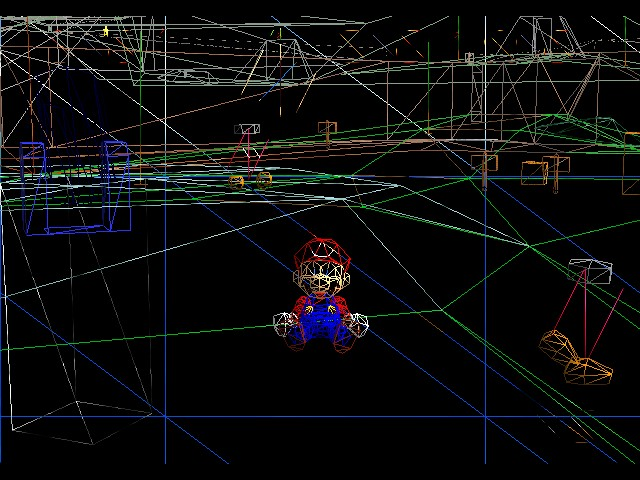
\includegraphics[width=0.8\textwidth]{images/m64wireframe.jpg}
            \caption{Super Mario 64 en mode fil de fer pour imager le \gls{vertex shader}}
            \label{fig:sm64_wireframe}
        \end{subfigure}
        \begin{subfigure}{0.5\textwidth}
            \centering
            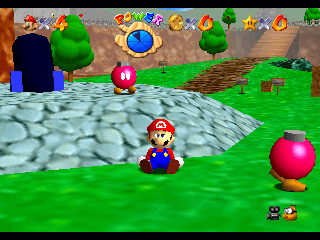
\includegraphics[width=0.8\textwidth]{images/m64result.png}
            \caption{Super Mario 64, après le passage par le \gls{fragment shader}}
            \label{fig:sm64_result}
        \end{subfigure}
        \caption{Exemple de rendu avec la stratégie de Silicon Graphics \cite{copetti_n64}}
        \label{fig:silicon_graphics_rendering}
    \end{figure}

    \newpage
    Enfin, le \gls{gpu} est de nouveau solicité pour le rendu de la scène
    finale, en utilisant les informations de la scène stockées dans le
    \gls{GBuffer} et en appliquant les effets de post-processing.
    Dans notre moteur, nous avons implémenté les techniques de rendu suivantes :
    \begin{multicols}{2}
    \begin{itemize}
        \item Le rendu différé
        \item Le rendu de la lumière en suivant le modèle de Phong 
        \item Le rendu des ombres en utilisant le \gls{shadow mapping}
        \item Le rendu de réflexions et de reflets en utilisant le \gls{ssr} (à but expérimental en utilisant le \gls{shader} de \emph{Imanol Fotia} \cite{imanolfotia})
        \item Le rendu d'occlusion ambiante en utilisant le \gls{ssao}
        \item Le rendu d'éblouissement en utilisant le \gls{bloom}
        \item L'anti-aliasing en utilisant le \gls{smaa}
    \end{itemize}
    \end{multicols}

    Une grande partie de ces techniques sont inspirées des travaux de Joey de Vries
    dans son site web LearnOpenGL \cite{learnopengl}, auquels nous avons
    ajouté des améliorations et des optimisations pour notre moteur grâce
    aux travaux de Adrian Courrèges sur DOOM 2016 \cite{courreges_doom2016}.
    \\ \\
    Pour un aperçu de la pipeline graphique de notre moteur, voir la section
    \ref{sec:graphics_pipeline}.

\subsubsection{Conception du moteur de physique}

    Le moteur de physique est responsable de la gestion des collisions et
    des interactions entre les objets de la scène. Il utilise un système de
    détection de collisions basé sur des formes géométriques simples, comme
    des sphères, des boîtes aux transformations non uniforme, des plans, etc.
    \\ \\
    La physique est ensuite calculée en utilisant une approche simplifiée des
    équations \emph{cinématiques} et des équations du \emph{principe fondamental de la dynamique}
    (\emph{deuxième loi de Newton}).

    \newpage

    Soit deux objets rigides, \( A \) et \( B \), se déplacent et entrent
    en collision. Voici comment nous calculons la réponse à la collision
    en utilisant les concepts de base de la physique des corps rigides.

    \begin{multicols}{2}

        \paragraph{Norme de la collision}
        La norme de la collision entre les deux corps est donnée par un vecteur
        normal à la surface de collision. Si les corps ont une normale de
        collision définie, cette norme est utilisée dans les calculs suivants.
    
        \nomenclature{$\mathbf{n}$}{Vecteur normal à la surface de collision}
        \nomenclature{$\mathbf{\lambda}_A$}{Normale de l'objet $A$}
        \nomenclature{$\mathbf{\lambda}_B$}{Normale de l'objet $B$}
        
        \begin{equation}
        \mathbf{n} = \mathbf{\lambda}_A \cdot \mathbf{\lambda}_B
        \end{equation}
    
        \paragraph{Vitesse relative}
        La vitesse relative des deux objets rigides \( A \) et \( B \) est calculée
        comme la différence entre leurs vitesses respectives :
    
        \nomenclature{$\mathbf{v}_{\text{relative}}$}{Vitesse relative entre deux objets}
        \nomenclature{$\mathbf{v}_A$}{Vitesse de l'objet $A$}
        \nomenclature{$\mathbf{v}_B$}{Vitesse de l'objet $B$}
        
        \begin{equation}
        \mathbf{v}_{\text{relative}} = \mathbf{v}_B - \mathbf{v}_A
        \end{equation}
    
        \paragraph{Vitesse relative selon la direction normale}
        \nomenclature{$v_{\text{normal}}$}{Vitesse relative projetée sur la normale de collision}
        
        \begin{equation}
        v_{\text{normal}} = \mathbf{v}_{\text{relative}} \cdot \mathbf{n}
        \end{equation}
    
        \paragraph{Coefficient de restitution (élasticité de la collision)}
        \nomenclature{$e$}{Coefficient de restitution}
        
        \begin{equation}
        e = 0.02
        \end{equation}
    
        \columnbreak
    
        \paragraph{Calcul de l'impulsion}
        \nomenclature{$I_{scalaire}$}{Quantité scalaire représentant l'impulsion échangée}
        \nomenclature{$m_A$}{Masse de l'objet $A$}
        \nomenclature{$m_B$}{Masse de l'objet $B$}
        
        \begin{equation}
        I_{scalaire} = \frac{(1 + e) \cdot v_{\text{normal}}}{m_A^{-1} + m_B^{-1}}
        \end{equation}
    
        \paragraph{Calcul du vecteur d'impulsion}
        \nomenclature{$\mathbf{I}$}{Vecteur d'impulsion appliqué pendant la collision}
        
        \begin{equation}
        \mathbf{I} = I_{scalaire} \cdot \mathbf{n}
        \end{equation}
    
        \paragraph{Application de l'impulsion et du couple}
        \nomenclature{$\mathbf{r}_A$}{Vecteur du centre de masse de $A$ au point d’impact}
        \nomenclature{$\mathbf{r}_B$}{Vecteur du centre de masse de $B$ au point d’impact}
        \nomenclature{$\mathbf{C}_A$}{Centre de masse de $A$}
        \nomenclature{$\mathbf{C}_B$}{Centre de masse de $B$}
        \nomenclature{$\mathbf{P}_{\text{impact}}$}{Point d’impact}
        
        \begin{equation}
        \mathbf{r}_A = \mathbf{P}_{\text{impact}} - \mathbf{C}_A
        \end{equation}
        \begin{equation}
        \mathbf{r}_B = \mathbf{P}_{\text{impact}} - \mathbf{C}_B
        \end{equation}
        \begin{equation}
        \text{Couple sur A} = \mathbf{r}_A \times \mathbf{I}
        \end{equation}
        \begin{equation}
        \text{Couple sur B} = \mathbf{r}_B \times \mathbf{I}
        \end{equation}
    
        \paragraph{Application de l'impulsion}
        \nomenclature{$\mathbf{v}_A'$}{Nouvelle vitesse de l’objet $A$}
        \nomenclature{$\mathbf{v}_B'$}{Nouvelle vitesse de l’objet $B$}
        
        \begin{equation}
        \mathbf{v}_A' = \mathbf{v}_A + \mathbf{I} \cdot m_A^{-1}
        \end{equation}
        \begin{equation}
        \mathbf{v}_B' = \mathbf{v}_B - \mathbf{I} \cdot m_B^{-1}
        \end{equation}
    
        \paragraph{Correction de la pénétration}
        \nomenclature{$\delta$}{Profondeur de pénétration}
        \nomenclature{$\mathbf{C}$}{Correction appliquée pour compenser la pénétration}
        \nomenclature{$\mathbf{P}_A$}{Position initiale de l'objet $A$}
        \nomenclature{$\mathbf{P}_B$}{Position initiale de l'objet $B$}
        \nomenclature{$\mathbf{P}_A'$}{Nouvelle position de l'objet $A$}
        \nomenclature{$\mathbf{P}_B'$}{Nouvelle position de l'objet $B$}
        
        \[
        \mathbf{C} = \delta \cdot \mathbf{n}
        \]
        \begin{equation}
        \mathbf{P}_A' = \mathbf{P}_A - \mathbf{C}
        \end{equation}
        \begin{equation}
        \mathbf{P}_B' = \mathbf{P}_B + \mathbf{C}
        \end{equation}
    
        \paragraph{Calcul du couple et de l'inertie}
        \nomenclature{$\mathbf{I}_{\text{locale}}$}{Matrice d’inertie locale}
        \nomenclature{$w$}{Largeur de l'objet}
        \nomenclature{$h$}{Hauteur de l'objet}
        \nomenclature{$d$}{Profondeur de l'objet}
    
        \begin{equation}
        \mathbf{I}_{\text{locale}} = \frac{m}{12} \begin{bmatrix} h^2 + d^2 & 0 & 0 \\ 0 & w^2 + d^2 & 0 \\ 0 & 0 & w^2 + h^2 \end{bmatrix}
        \end{equation}
    
        \paragraph{Accélération angulaire}
        \nomenclature{$\mathbf{\alpha}$}{Accélération angulaire}
        \nomenclature{$\mathbf{T}$}{Couple appliqué}
        \nomenclature{$\mathbf{I}^{-1}$}{Inverse de la matrice d’inertie}
        
        \begin{equation}
        \mathbf{\alpha} = \mathbf{I}^{-1} \cdot \mathbf{T}
        \end{equation}
    
    \end{multicols}

\subsubsection{Conception de l'arbre de données}

    Dans notre moteur, nous avons choisi d'utiliser un arbre de données
    pour représenter la scène 3D. Cet arbre est composé de n\oe{}uds, où
    chaque n\oe{}ud représente un objet de la scène. Chaque n\oe{}ud
    contient des informations sur la position, la rotation et l'échelle de
    l'objet, ainsi que des références vers ses enfants et son père.
    Cela permet de créer une hiérarchie d'objets, où chaque objet peut
    être transformé indépendamment tout en étant affecté par les
    transformations de ses parents.
    \\ \\
    Ce modèle d'arbre de données est inspiré du moteur de jeu Godot, qui
    utilise également un arbre de n\oe{}uds pour représenter une scène.
    \\ \\
    Les n\oe{}uds de l'arbre sont génériques, ce qui garantit un stockage
    efficace des données et une gestion facile des objets de la scène (figure \ref{fig:node_structure}).

    \begin{figure}[h]
        \centering
        \includesvg[width=\linewidth]{images/node.svg}
        \emph{La structure présentée ici est une simplification de la structure utilisée dans notre moteur de jeu.}
        \caption{Structure d'un noeud générique}
        \label{fig:node_structure}
    \end{figure}

    Vous pouvez vous référer à la table \ref{tab:raptiquax_nodes} pour découvrir
    les différents types de n\oe{}uds que nous avons implémentés dans notre
    moteur de jeu. Chaque n\oe{}ud est responsable d'un aspect spécifique de
    la scène, ce qui permet de créer un tout cohérent et fluide.


\subsubsection{Conception des classes et héritage}

    Pour assurer une bonne organisation du code et une gestion efficace
    des objets de la scène, nous avons utilisé un système de classes capable
    de gérer l'héritage.
    \\ \\
    Le code source du moteur est précompilé par un outil développé par nos
    soins, qui permet de générer un code source en C à partir d'un fichier
    classe inspiré de la syntaxe de \emph{C++}. Les classes ainsi générées
    sont ensuites liées entre elles par un header de liaison, lui aussi
    généré par l'outil. Cela permet de créer un code source propre et
    facilement lisible, tout en assurant une bonne gestion de la mémoire et des
    performances.
    \\ \\
    Un exemple des classes utilisées par l'outil de précompilation est
    présenté dans le listing \ref{lst:class_template}.
    \\ \\
    Le code source généré utilise les arguments variadiques et prend en charge
    les promotions automatiques des types.
\subsubsection{Conception des entrées sorties}

    Le moteur prend en charge les entrées/sorties de sorte à permettre
    aux développeurs de créer des jeux en utilisant des fichiers de
    ressources sans avoir à se soucier de l'implémentation ou de la gestion
    de la mémoire et des performances.
\paragraph{Chargement des ressources}

    Les ressources du moteurs sont chargées à l'aide de diverses
    fonctions d'entrée/sortie, qui permettent de charger des fichiers
    de différents formats. Voici une liste non exhaustive des formats
    de fichiers pris en charge par le moteur :\\
    \begin{itemize}
        \item \textbf{OBJ} : format de fichier 3D utilisé pour stocker
        des modèles 3D. Il est simple et largement utilisé dans
        l'industrie du jeu vidéo. \cite{obj_format}
        \item \textbf{PNG} : format de fichier image utilisé pour stocker
        des textures.
        \item \textbf{JPG} : format de fichier image compressé utilisé pour stocker
        des textures.
        \item \textbf{WAV} : format de fichier audio brut utilisé pour stocker
        des sons.
        \item \textbf{OGG} : format de fichier audio compressé utilisé généralement pour
        stocker des sons.
        \item \textbf{MP3} : format de fichier audio compressé utilisé généralement pour
        stocker des musiques.
        \item \textbf{SCENE} : format de fichier propriétaire utilisé pour
        stocker des scènes 3D.
        \item \textbf{FS} : format de fichier shader utilisé pour stocker
        des shaders de fragment. \cite{glsl}
        \item \textbf{VS} : format de fichier shader utilisé pour stocker
        des shaders de vertex. \cite{glsl}\\
    \end{itemize}
    
    Les ressources sont stockées en cache pour éviter de les recharger
    plusieurs fois. Le moteur utilise un système de gestion de
    ressources qui permet de charger et de décharger les ressources
    du cache sur demande. Cela permet de réduire la consommation de mémoire et
    d'optimiser les performances du moteur.
\paragraph{Communication en réseau (SocketIO)}

    Le moteur permet en outre de gérer la communication en réseau entre
    des clients et un serveur en multithreads. Pour cela, nous avons utilisé
    la librairie \emph{Socket} en C, qui permet de gérer la communication en
    temps réel entre le serveur et les clients.
    Nous avons implémenté un serveur Socket qui gère les connexions des
    clients et les messages échangés entre eux. Le serveur est capable de
    gérer plusieurs clients en même temps et de leur envoyer des messages
    en temps réel. Il est également capable de gérer les connexions et
    déconnexions des clients, ainsi que les erreurs de communication.
    Le serveur de démonstration que nous avons mis en place est capable de
    gérer une dizaine de commandes différentes (table \ref{tab:raptiquax_requests}).
    \\ \\
    Comme preuve de concept, nous avons mis en place un serveur pour \og \emph{FPS Chess} \fg{}, un
    mini-jeu fps multijoueur qui gère plusieurs parties de deux joueurs en même temps.

\subsection{Création des ressources}
\subsubsection{Conception du modèle 3d et des textures}
La map du jeu, représentant le bâtiment Claude Chappe et ses
environs, a été créée en plusieurs étapes via Blender : \\ \\
\textbf{- Modélisation 3D des modèles :} \\
\\
On utilise des objets préfabriqués de Blender, modifiables
grâce à divers outils pour obtenir les formes désirées (ex :
transformation d'un cube en mur ou en porte comme on le voit
figure ~\ref{fig:cube-base} et ~\ref{fig:cube-modif}). Nous
avons d'abord modélisé la structure de base du bâtiment, puis
ajouté des éléments exclusifs au jeu, comme des trous dans le
sol et les murs pour un parcours de poursuite, ainsi que trois
salles secrètes avec des ordinateurs pour les mini-jeux.\\

\textbf{- Normals :} \\\\
Les normales définissent l'orientation des faces des objets et
influencent l'effet de la lumière. Bien que généralement correctes
par défaut, il est parfois nécessaire de les ajuster pour éviter
des erreurs d'affichage. \\

\textbf{- Texturage :} \\ \\
Une fois les objets modélisés, ils sont texturés en utilisant des
textures d’image ou des couleurs unies, compatibles avec le
moteur 3D. Par exemple, une porte est texturée en rouge uni,
tandis que les murs utilisent une texture image de plastique
gris/blanc.\\

\textbf{- Séparation des zones :} \\

Les objets sont regroupés en "collections" selon leur emplacement
(amphithéâtre, couloirs, salles de classe, etc.), ce qui facilite
leur exportation en fichiers .obj distincts et optimise le
chargement des ressources dans le moteur.\\

\textbf{- Optimisation des modèles et textures :} \\

Les erreurs de modélisation sont corrigées pour garantir une
bonne intégration. Les UV Maps des textures sont ajustées pour
assurer un affichage correct après l'exportation.\\

\textbf{- Exportation :} \\

Les objets d’une zone sont fusionnés (JOIN) pour simplifier
l’importation dans le moteur (un seul objet au lieu de plusieurs
centaines). On les exporte ensuite en .obj et .mtl (textures), en
veillant à inclure toutes les images de textures nécessaires.

\begin{figure}
    \centering
    \begin{minipage}{0.49\linewidth}
        \centering
        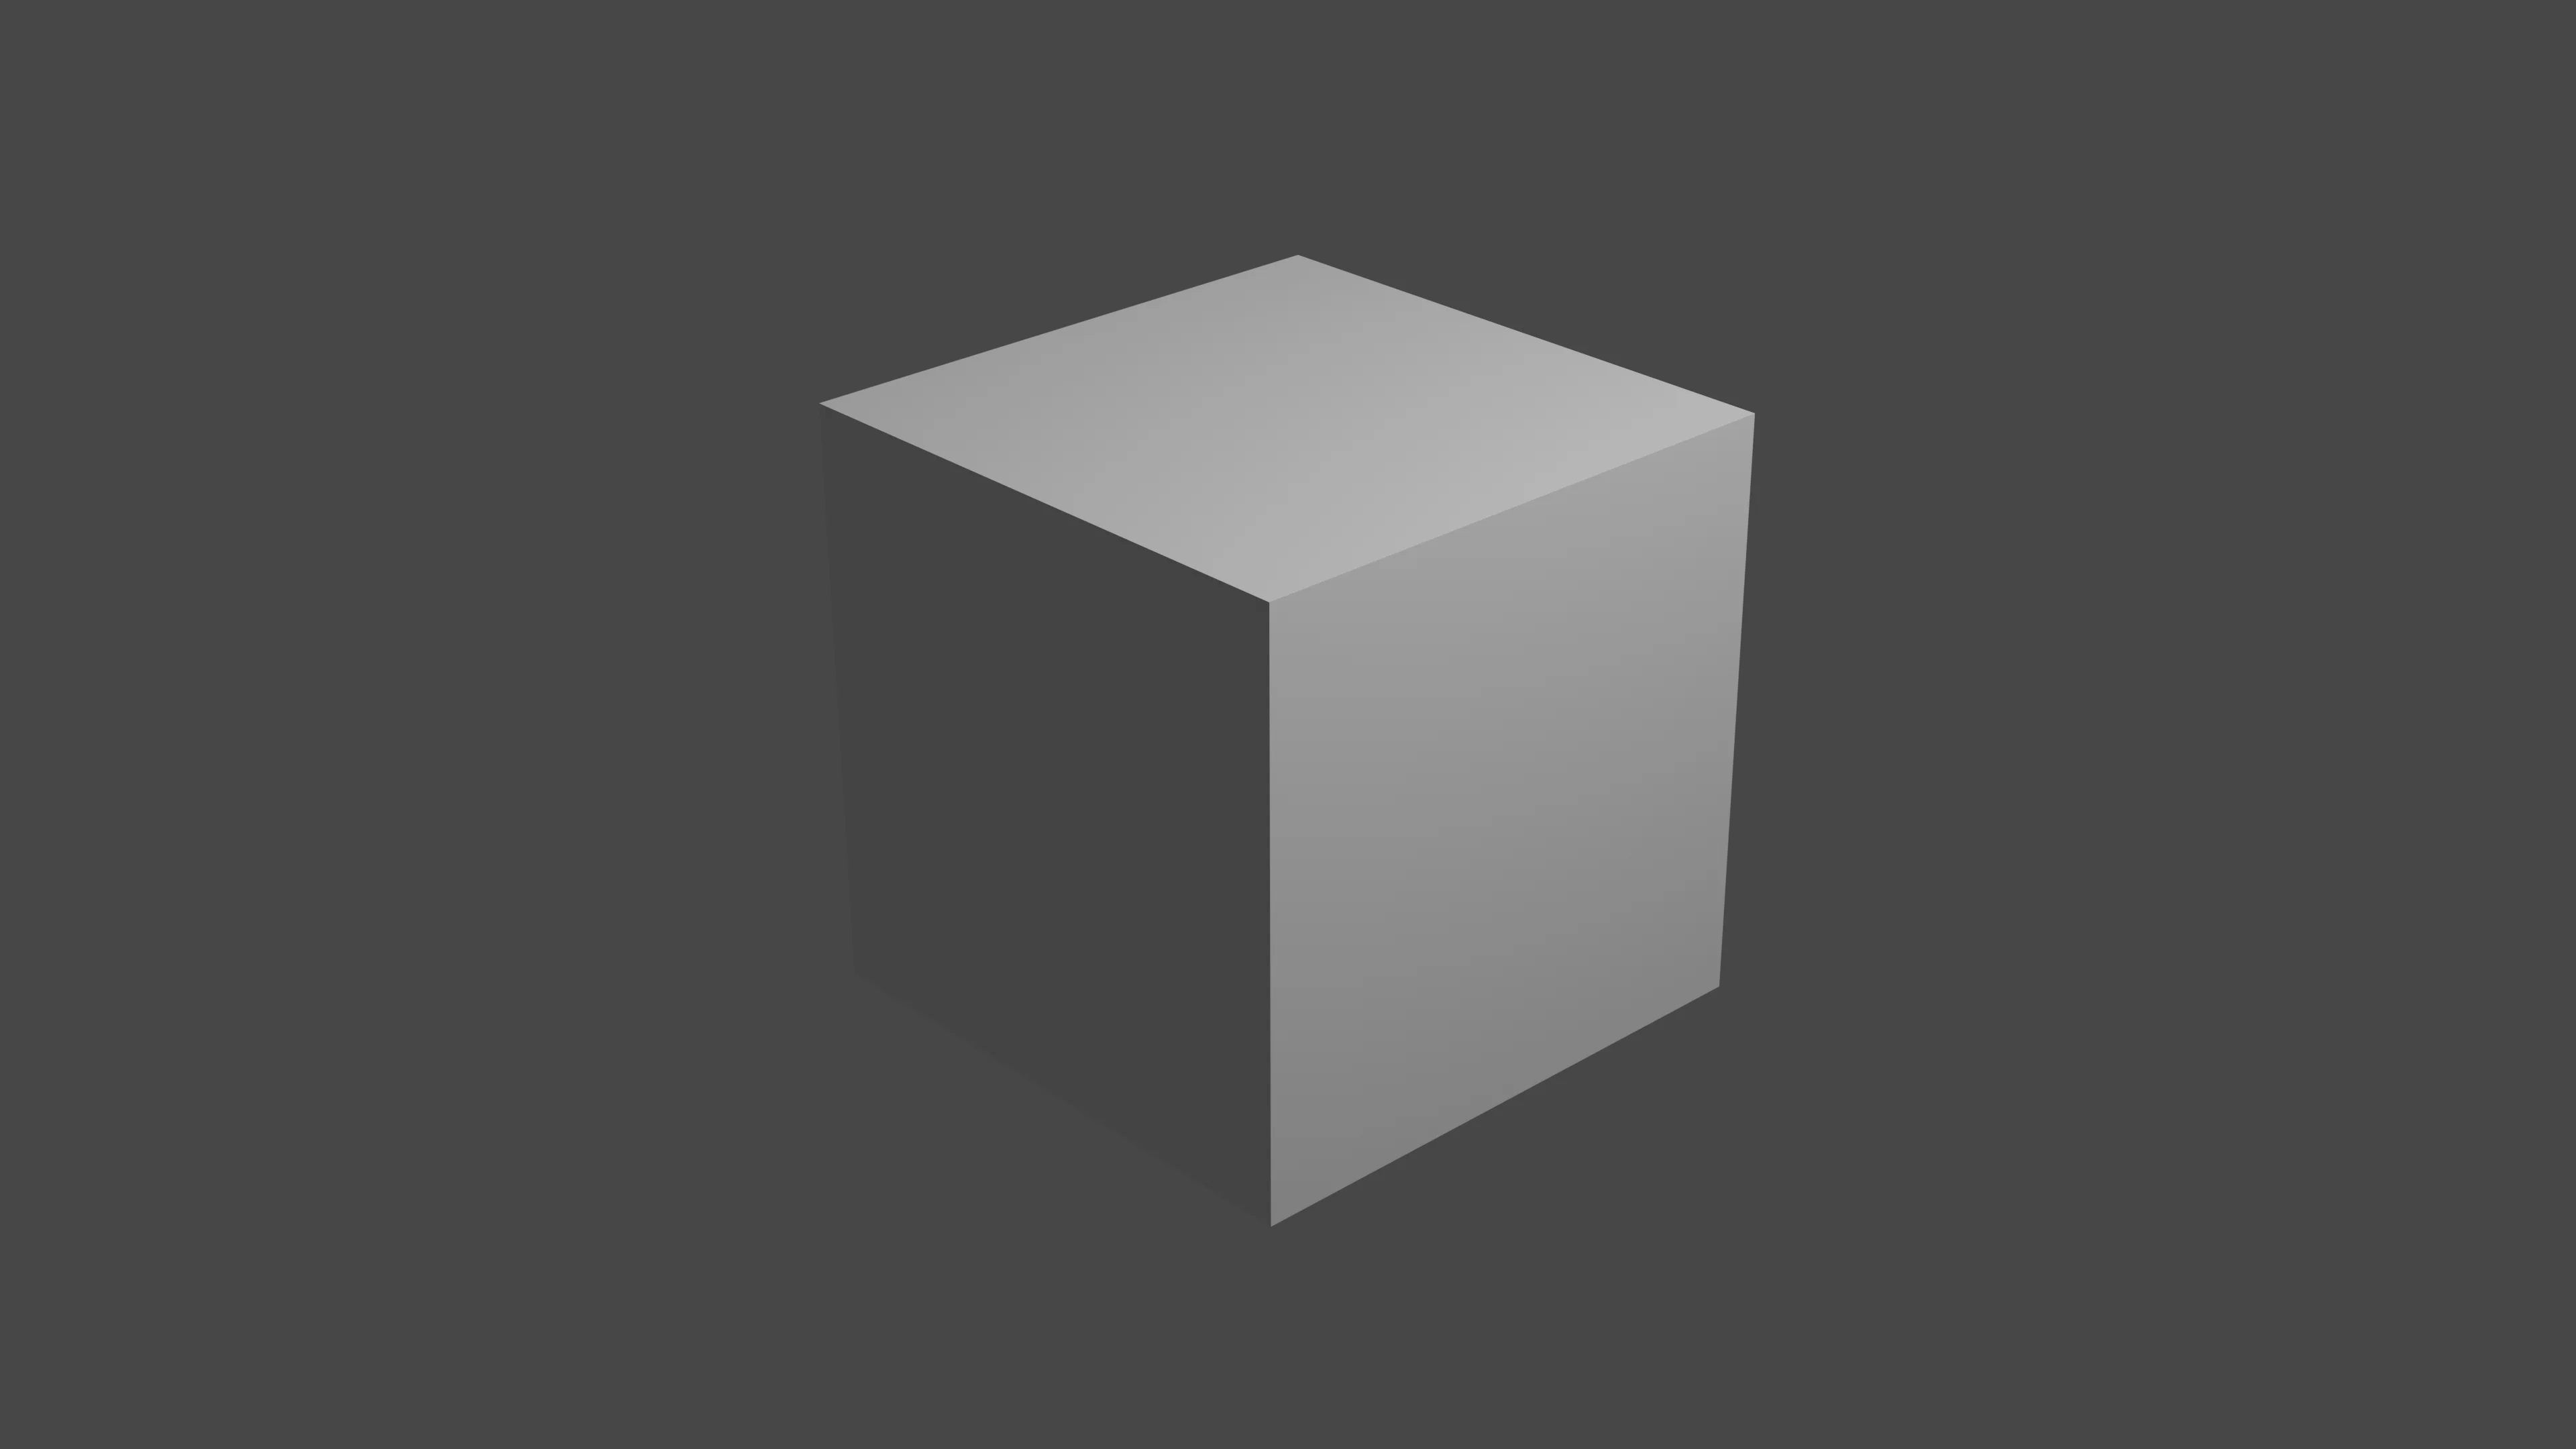
\includegraphics[width=\linewidth]{images/base_cube.png}
        \caption{Cube de base Blender}
        \label{fig:cube-base}
    \end{minipage}
    \hfill
    \begin{minipage}{0.49\linewidth}
        \centering
        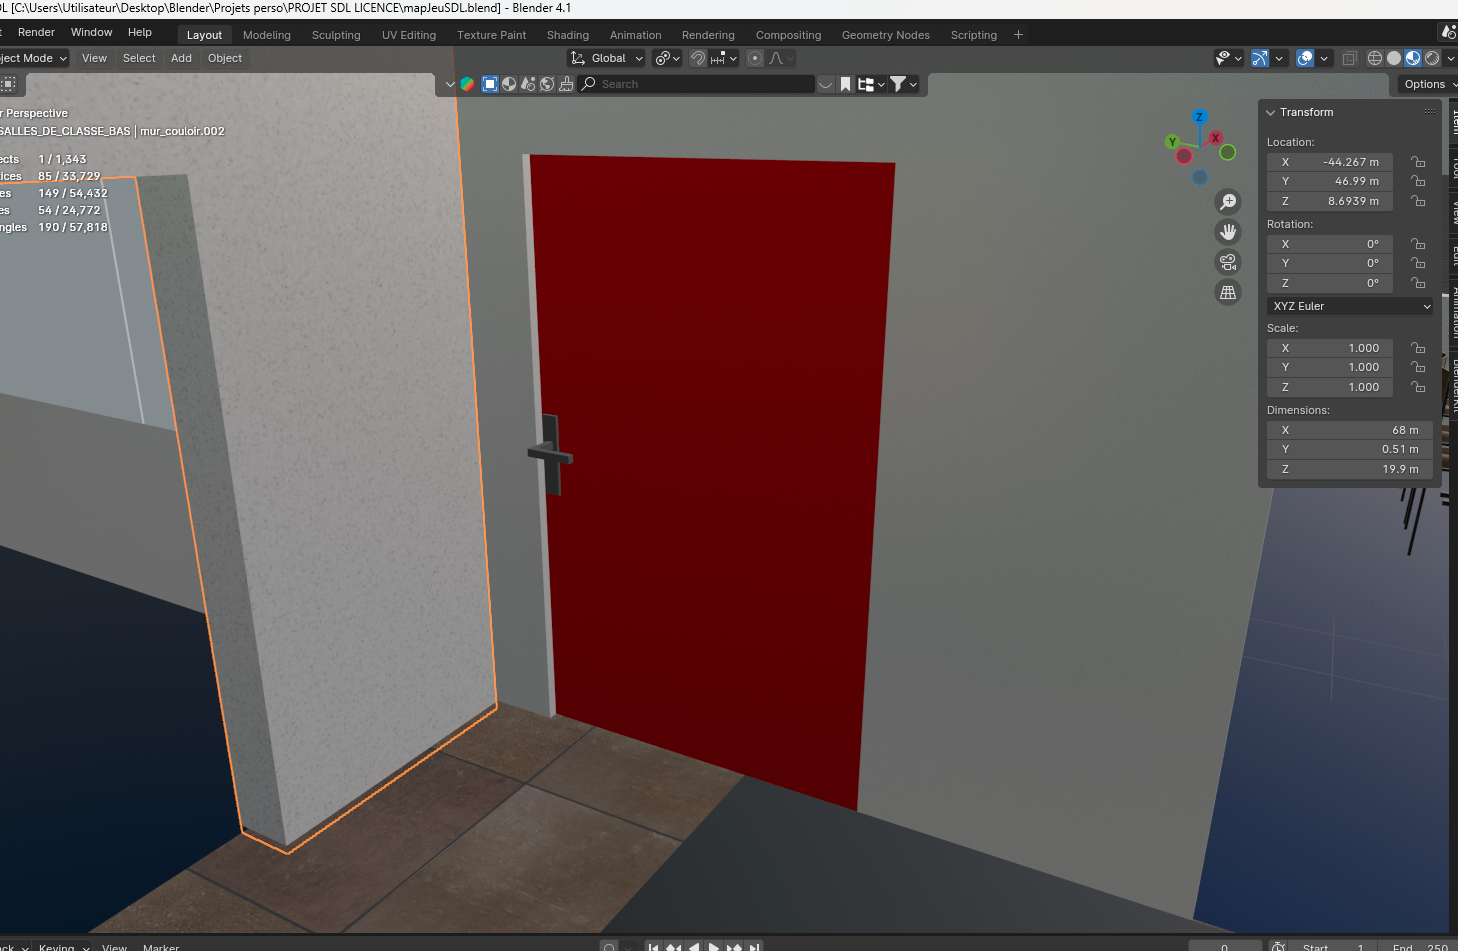
\includegraphics[width=\linewidth]{images/cubemodif.png}
        \caption{Cubes modifiés en divers objets}
        \label{fig:cube-modif}
    \end{minipage}
\end{figure}
\subsubsection{Conception des musiques et effets sonores}

Les musiques et les effets sonores sont tous les deux composés
sur le logiciel FL Studio.\\\\
\textbf{- Conception des musiques :}\\\\
À partir de sons déjà existants (libres de droits), on les
utilise en les modifiant (ou non), pour en faire des mélodies
(à l'aide d'un clavier synthétiseur), des boucles de divers instruments,
bref créer une musique.\\\\
\textbf{- Conception des effets sonores :}\\\\
Pour les effets sonores, on utilise à nouveau des sons déjà
existants, évidemment sans faire des mélodies cette fois. On les
modifie à travers divers plugins du logiciel (pitch grave/aigu,
réverbération, etc.).\\
Vous trouverez en annexe un exemple de composition musicale (voir figure \ref{fig:flstudio.png}).
\subsection{Gestion des scènes}
\subsubsection{Gestion des objets}

Les objets sont des entités gérées par des scripts importés dans les scènes du
moteur 3D.
\\ \\
Les scripts sont écrits en C et sont chargés par le moteur 3D au moment de
l'importation de la scène. Ils sont ensuite exécutés par le moteur 3D lors de
la boucle de jeu à des instants clés.
\\ \\
On peut ainsi définir des comportements spécifiques pour l'initialisation
des objets, leur mise à jour et lors de la réception de signaux.
\\ \\
Les interactions entre les objets et l'environnement sont gérées par ces
signaux qui sont émis notamment lorsque les objets entrent en collision avec
d'autres objets, mais il est possible de paramétrer divers signaux personnalisés.

\paragraph{Mini-jeux}
Dans le cadre de Chapper's Fallout, un mini-jeu en 2D a été conçu pour s’intégrer de manière fluide à l’univers 
du jeu principal. Ce mini-jeu est accessible via un unique ordinateur interactif placé dans le bâtiment. Lorsqu’il 
est activé, une fenêtre s’ouvre, simulant le démarrage d’un système d’exploitation. Cette interface, gérée par un 
système de fenêtrage complet, lance automatiquement un bureau virtuel et orchestre les différentes scènes via un 
gestionnaire d’événements centralisé.
\\
Le cœur de ce mini-jeu repose sur une séquence dynamique dans laquelle le joueur incarne un petit personnage à l’écran. 
L’objectif est simple mais engageant : survivre pendant un certain temps en esquivant des boules de feu tombant aléatoirement 
du ciel. L’ensemble est enrichi par quelques animations et effets visuels qui donnent vie à l’interface et renforcent 
l’immersion dans cet environnement fictif d’ordinateur.
\\
Sur le plan technique, la gestion des événements est assurée par une boucle principale qui interroge SDL en temps réel pour 
capter les entrées utilisateur (clics, mouvements de souris, frappes clavier). Le mini-jeu dispose de son propre « event manager », 
qui gère les transitions entre les différentes scènes et assure la réactivité du gameplay.
\\
Le système de fenêtres permet la création, la mise à jour et la destruction d’interfaces graphiques synchronisées avec les 
événements du jeu, garantissant une expérience utilisateur fluide et cohérente.
\\
Enfin, les structures de données, notamment celles associées aux éléments du bureau et aux textures animées, jouent un rôle clé dans 
l’affichage dynamique. Par exemple, la mise à jour des sprites utilise un compteur de frames pour sélectionner la portion adéquate 
d’un spritesheet, assurant ainsi une animation fluide. Ce modèle est pensé pour être facilement extensible, permettant l’ajout de 
nouveaux comportements ou scènes sans compromettre l’équilibre général du système.
\\
Dans l’ensemble, cette architecture modulaire, fondée sur un système de fenêtres intégré et une gestion rigoureuse des événements, 
permet d’offrir un mini-jeu simple mais immersif, parfaitement intégré à l’expérience globale de Chapper's Fallout.
\\
Cependant, en raison de difficultés techniques rencontrées lors de son intégration dans la scène principale, le mini-jeu ne sera 
finalement pas accessible via l’ordinateur en jeu. Il sera uniquement jouable via une touche spéciale au lancement du jeu, permettant 
d’y accéder directement en dehors du gameplay principal.
\\
\subsubsection{Gestion des PNJ (personnages non joueurs)}

Les PNJ sont des entités qui se déplacent dans la scène. Ils sont gérés par le moteur
3D et sont placés dans la scène via l'éditeur de niveau. Leurs comportements sont
défini par des scripts qui sont exécutés par le moteur et utilisent le principe
de la machine à état.\\

Pour rendre les PNJ plus réalistes, nous avons implémenté un système de chemins
de navigation. Ce système permet aux PNJ de se déplacer le long d'un chemin prédéfini
dans la scène. Les chemins sont définis par des points de contrôle placés dans
la scène. Le moteur 3D utilise ces points de contrôle pour calculer la trajectoire
des PNJ et les faire se déplacer le long de cette trajectoire.

\subsubsection{Placement des collisions}
Une fois que le modèle est affiché et que tous les obstacles et éléments de
décors sont placés, il faut qu'on puisse intéragir avec eux.
\\ \\
Pour éviter de passer à travers les murs il faut detecter quand le joueur
est à la même position que le mur en question.
\\ \\
On a choisi d'abord d'afficher le modèle 3D, ensuite grâce à l'éditeur on
place des "boites" de collisions. En jeu ces boîte seront invisible, mais
infranchissable, ça permet de ne pas traverser les obstacles.
\\ \\
Par exemple on modelise une table avec le moteur 3D. Dans l'éditeur on rajoute
manuellement une "boite" de collisions à l'emplacement de la table, on cherche
à épouser la forme de la table. En jeu on verra que la table, et on ne pourra
pas la traverser, on peut même monter dessus etc.
\\ \\
Sur la figure \ref{fig:fig2} montre les différents types de "boîtes" On voit qu'on dessine
chaque éléments avec des boîtes.



\begin{figure}[H]
    \centering
    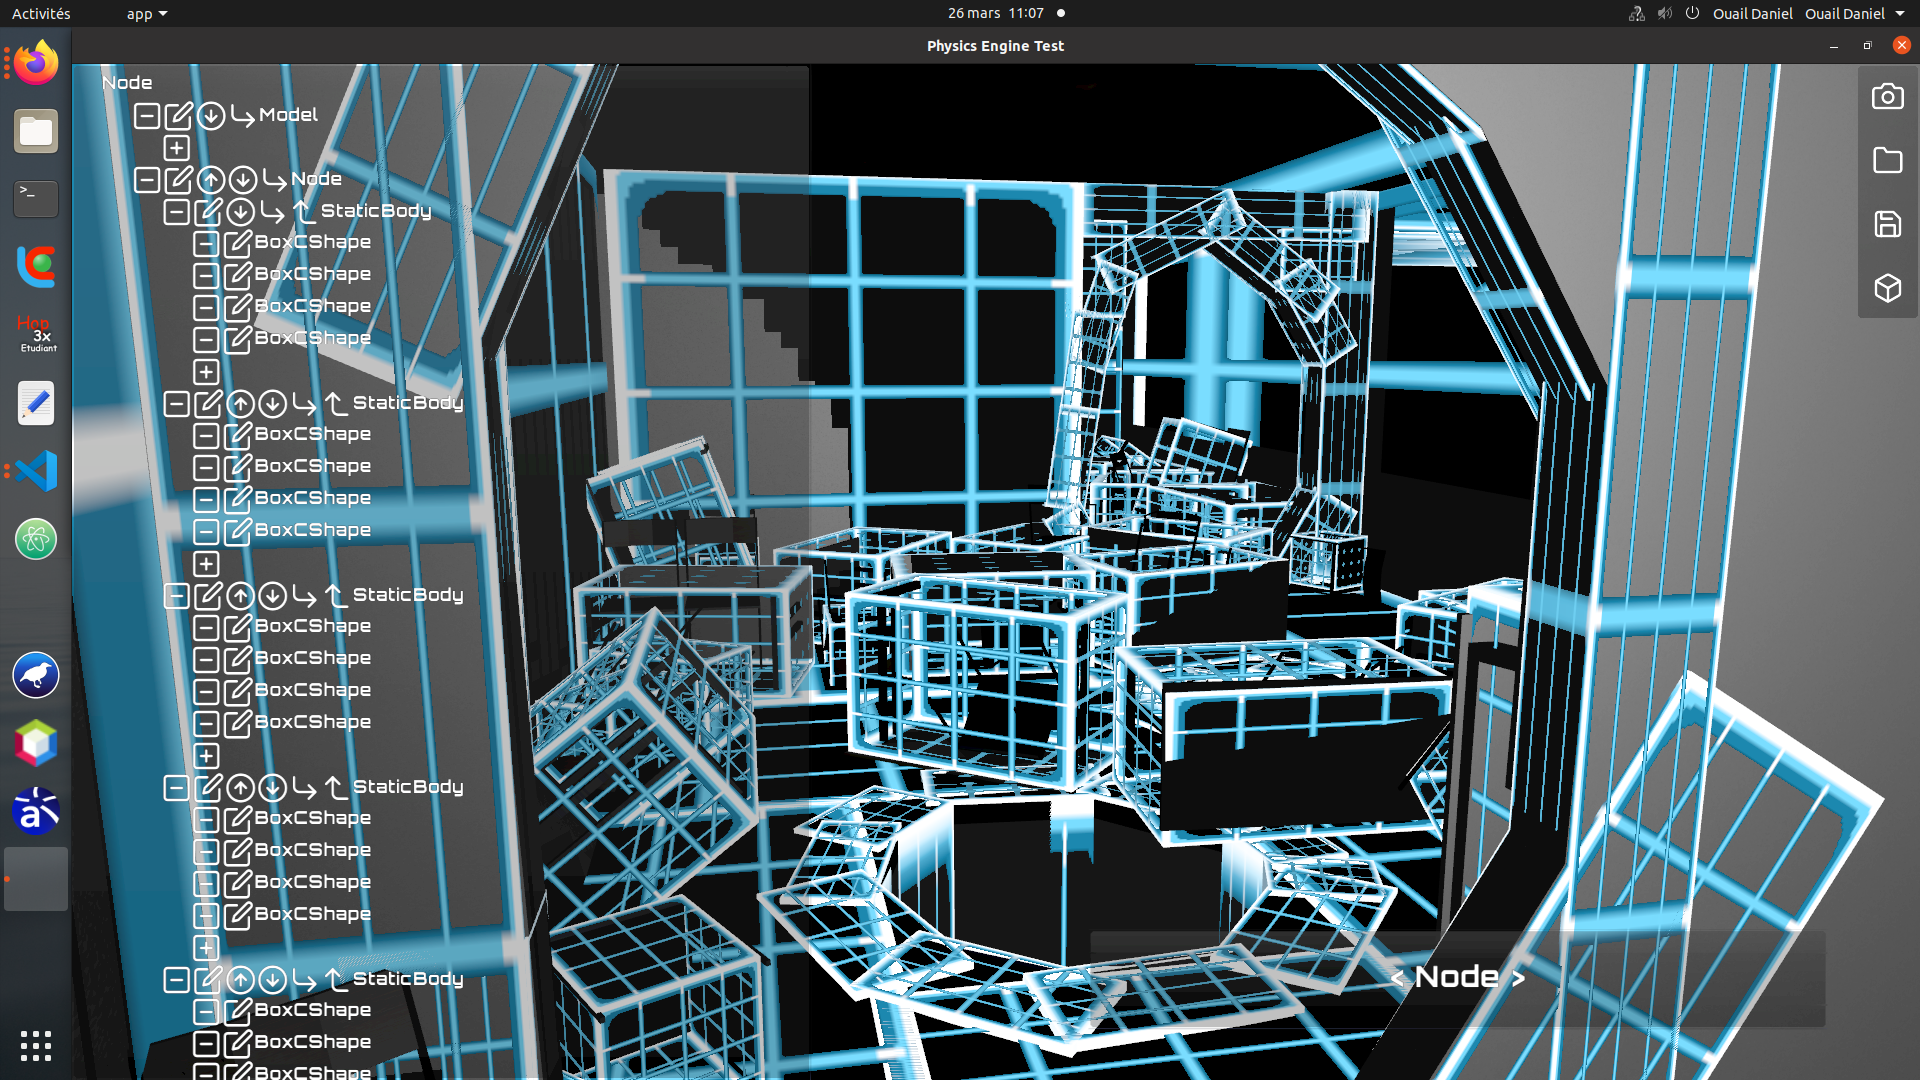
\includegraphics[width=1\linewidth]{images/screenshot_editeur.png}
    \caption{Capture d'écran de l'éditeur de niveau}
    \label{fig:fig2}
\end{figure}

Les coordonnées de chaque boîtes de collisions sont enregistrées avec l'éditeur
dans un fichier .scene, ce fichier sera lu au moment de l'execution pour
charger le modèle et les collisions.



\newpage

\section{Résultats et conclusion}
\section{Bibliographie}
\printglossaries
\printnomenclature
\begin{thebibliography}{9}
    \bibitem{soniccoloru}
    Sonic Team (3 septembre 2021) \emph{Sonic Colours Ultimate}, SEGA.
    
    \bibitem{learnopengl} 
    Joey de Vries, \textit{LearnOpenGL}.  
    Disponible en ligne : \url{https://learnopengl.com/}.  
    LearnOpenGL est une ressource en ligne exhaustive dédiée à l'apprentissage de la programmation graphique avec OpenGL.  
    Le site couvre des sujets tels que la manipulation des shaders, la gestion des textures, les transformations 3D,  
    ainsi que des concepts avancés comme le rendu différé et les ombres en temps réel.  
    Consulté le 1 avril 2025.

    \bibitem{imanolfotia} 
    Imanol Fotia, \textit{Blog - Article 1}.  
    Disponible en ligne : \url{https://imanolfotia.com/blog/1}.  
    Ce blog aborde divers sujets liés à la programmation, à l'ingénierie logicielle et aux technologies modernes.  
    Il propose des analyses approfondies, des tutoriels techniques et des réflexions sur les bonnes pratiques en développement.  
    Consulté le 1 avril 2025.

    \bibitem{iehl_deferred_vs_forward} 
    Jean-Claude Iehl, \textit{Deferred Shading vs Forward Shading}.  
    Disponible en ligne : \url{https://perso.univ-lyon1.fr/jean-claude.iehl/Public/educ/M2PROIMA/2018/deferred_vs_forward.html}.  
    Ce document pédagogique explique les différences entre le rendu différé (Deferred Shading) et le rendu direct (Forward Shading).  
    Il couvre les principes fondamentaux de chaque technique, leurs avantages et inconvénients, ainsi que leurs applications  
    dans les moteurs de rendu modernes.  
    Consulté le 1 avril 2025.

    \bibitem{courreges_doom2016} 
    Adrian Courrèges, \textit{DOOM (2016) - Graphics Study}.  
    Disponible en ligne : \url{https://www.adriancourreges.com/blog/2016/09/09/doom-2016-graphics-study/}.  
    Cet article propose une analyse approfondie du moteur graphique de *DOOM (2016)*, en explorant les techniques de rendu utilisées,  
    telles que le rendu différé, l'éclairage, la gestion des ombres, le post-traitement et l'optimisation des performances.  
    L'auteur décortique les effets visuels et les choix techniques ayant permis au jeu d'atteindre un haut niveau de fluidité et de qualité visuelle.  
    Consulté le 1 avril 2025.

    \bibitem{valve_source_engine} 
    Valve Corporation, \textit{Source Engine Features}.  
    Disponible en ligne : \url{https://developer.valvesoftware.com/wiki/Source_Engine_Features}.  
    Cette page du wiki officiel de Valve décrit les fonctionnalités du moteur Source, utilisé dans de nombreux jeux  
    comme *Half-Life 2*, *Portal* et *Counter-Strike: Source*. Elle couvre des aspects tels que le rendu graphique,  
    la gestion de la physique, le réseau, l'intelligence artificielle et les outils de développement fournis avec le moteur.  
    Consulté le 1 avril 2025.

    \bibitem{wikipedia_cryengine} 
    Wikipedia, \textit{CryEngine}.  
    Disponible en ligne : \url{https://en.wikipedia.org/wiki/CryEngine}.  
    Cet article de Wikipedia fournit une vue d'ensemble détaillée de CryEngine, un moteur de jeu développé par Crytek.  
    Il explore ses caractéristiques techniques, ses applications dans les jeux vidéo, ses versions successives et ses améliorations au fil du temps.  
    CryEngine est reconnu pour ses capacités de rendu photoréaliste et son utilisation dans des jeux populaires comme *Crysis*.  
    Consulté le 1 avril 2025.

    \bibitem{chanhaeng_normalparallax} 
    Chanhaeng, \textit{Normal/Parallax Mapping with Self-Shadowing}.  
    Disponible en ligne : \url{https://chanhaeng.blogspot.com/2019/01/normalparllax-mapping-with-self.html}.  
    Cet article explique en détail l'implémentation du normal mapping et du parallax mapping avec auto-ombrage.  
    L'auteur y décrit les concepts théoriques de ces techniques graphiques avancées et leur application dans les moteurs de rendu.  
    Le blog fournit également un code exemple pour implémenter ces effets dans les shaders.  
    Consulté le 1 avril 2025.

    \bibitem{silicon_graphics}
    Silicon Graphics.
    Disponible en ligne : \url{https://www.sgi.com/}.
    Silicon Graphics, Inc. (SGI) est une entreprise américaine spécialisée dans la conception de stations de travail et de superordinateurs.
    Pionnier dans le domaine de l'informatique graphique, elle est à l'origine de la création d'OpenGL,
    une API de rendu 2D et 3D largement adoptée dans l'industrie. Leur modèle de pipeline graphique a influencé
    de nombreux moteurs de jeu modernes, ayant fait ses preuves dans l'industrie du jeu vidéo lors de leur collaboration avec
    Nintendo en 1996 pour la création de la Nintendo 64 \cite{copetti_n64}.

    \bibitem{copetti_n64} 
    Fabio Copetti, \textit{Nintendo 64}.  
    Disponible en ligne : \url{https://www.copetti.org/writings/consoles/nintendo-64/}.  
    Cet article offre une analyse détaillée de la console Nintendo 64, y compris son architecture matérielle, ses composants, et les défis techniques rencontrés lors de son développement.  
    L'auteur explore également les innovations apportées par la N64, comme le processeur graphique et le stockage sur cartouche.  
    Consulté le 1 avril 2025.

    \bibitem{lalanguefrancaise}
    La Langue Française.
    Disponible en ligne : \url{https://www.lalanguefrancaise.com/}.
    La Langue Française est un site dédié à la langue française, proposant des ressources, des articles et des outils pour améliorer la maîtrise de la langue.
    Il aborde divers sujets tels que la grammaire, le vocabulaire, l'orthographe et la culture francophone.
    Le site est une référence pour les francophones souhaitant approfondir leur connaissance de la langue française.

    \bibitem{obj_format}
    Wavefront Technologies, \textit{OBJ File Format}.
    Disponible en ligne : \url{https://en.wikipedia.org/wiki/Wavefront_.obj_file}.
    Le format de fichier OBJ est un format de fichier standard pour représenter des objets 3D.
    Il est largement utilisé dans l'industrie de la modélisation 3D et est pris en charge par de nombreux logiciels de modélisation.
    Le format OBJ est simple et facile à lire, ce qui en fait un choix populaire pour l'échange de données 3D entre différentes applications.
    Il permet de stocker des informations sur la géométrie et éventuellement des textures, des matériaux et d'autres attributs associés à un objet 3D s'il est
    accompagné d'un fichier MTL.

    \bibitem{glsl}
    Khronos Group, \textit{OpenGL Shading Language (GLSL)}.
    Disponible en ligne : \url{https://www.khronos.org/opengl/wiki/OpenGL_Shading_Language}.
    OpenGL Shading Language (GLSL) est un langage de
    programmation de shaders de haut niveau dont la syntaxe est fondée sur
    le langage C.
    

\end{thebibliography}
\newpage
\section{Annexes}

\printglossaries
\printnomenclature
\begin{thebibliography}{9}
    \bibitem{soniccoloru}
    Sonic Team (3 septembre 2021) \emph{Sonic Colours Ultimate}, SEGA.
    
    \bibitem{learnopengl} 
    Joey de Vries, \textit{LearnOpenGL}.  
    Disponible en ligne : \url{https://learnopengl.com/}.  
    LearnOpenGL est une ressource en ligne exhaustive dédiée à l'apprentissage de la programmation graphique avec OpenGL.  
    Le site couvre des sujets tels que la manipulation des shaders, la gestion des textures, les transformations 3D,  
    ainsi que des concepts avancés comme le rendu différé et les ombres en temps réel.  
    Consulté le 1 avril 2025.

    \bibitem{imanolfotia} 
    Imanol Fotia, \textit{Blog - Article 1}.  
    Disponible en ligne : \url{https://imanolfotia.com/blog/1}.  
    Ce blog aborde divers sujets liés à la programmation, à l'ingénierie logicielle et aux technologies modernes.  
    Il propose des analyses approfondies, des tutoriels techniques et des réflexions sur les bonnes pratiques en développement.  
    Consulté le 1 avril 2025.

    \bibitem{iehl_deferred_vs_forward} 
    Jean-Claude Iehl, \textit{Deferred Shading vs Forward Shading}.  
    Disponible en ligne : \url{https://perso.univ-lyon1.fr/jean-claude.iehl/Public/educ/M2PROIMA/2018/deferred_vs_forward.html}.  
    Ce document pédagogique explique les différences entre le rendu différé (Deferred Shading) et le rendu direct (Forward Shading).  
    Il couvre les principes fondamentaux de chaque technique, leurs avantages et inconvénients, ainsi que leurs applications  
    dans les moteurs de rendu modernes.  
    Consulté le 1 avril 2025.

    \bibitem{courreges_doom2016} 
    Adrian Courrèges, \textit{DOOM (2016) - Graphics Study}.  
    Disponible en ligne : \url{https://www.adriancourreges.com/blog/2016/09/09/doom-2016-graphics-study/}.  
    Cet article propose une analyse approfondie du moteur graphique de *DOOM (2016)*, en explorant les techniques de rendu utilisées,  
    telles que le rendu différé, l'éclairage, la gestion des ombres, le post-traitement et l'optimisation des performances.  
    L'auteur décortique les effets visuels et les choix techniques ayant permis au jeu d'atteindre un haut niveau de fluidité et de qualité visuelle.  
    Consulté le 1 avril 2025.

    \bibitem{valve_source_engine} 
    Valve Corporation, \textit{Source Engine Features}.  
    Disponible en ligne : \url{https://developer.valvesoftware.com/wiki/Source_Engine_Features}.  
    Cette page du wiki officiel de Valve décrit les fonctionnalités du moteur Source, utilisé dans de nombreux jeux  
    comme *Half-Life 2*, *Portal* et *Counter-Strike: Source*. Elle couvre des aspects tels que le rendu graphique,  
    la gestion de la physique, le réseau, l'intelligence artificielle et les outils de développement fournis avec le moteur.  
    Consulté le 1 avril 2025.

    \bibitem{wikipedia_cryengine} 
    Wikipedia, \textit{CryEngine}.  
    Disponible en ligne : \url{https://en.wikipedia.org/wiki/CryEngine}.  
    Cet article de Wikipedia fournit une vue d'ensemble détaillée de CryEngine, un moteur de jeu développé par Crytek.  
    Il explore ses caractéristiques techniques, ses applications dans les jeux vidéo, ses versions successives et ses améliorations au fil du temps.  
    CryEngine est reconnu pour ses capacités de rendu photoréaliste et son utilisation dans des jeux populaires comme *Crysis*.  
    Consulté le 1 avril 2025.

    \bibitem{chanhaeng_normalparallax} 
    Chanhaeng, \textit{Normal/Parallax Mapping with Self-Shadowing}.  
    Disponible en ligne : \url{https://chanhaeng.blogspot.com/2019/01/normalparllax-mapping-with-self.html}.  
    Cet article explique en détail l'implémentation du normal mapping et du parallax mapping avec auto-ombrage.  
    L'auteur y décrit les concepts théoriques de ces techniques graphiques avancées et leur application dans les moteurs de rendu.  
    Le blog fournit également un code exemple pour implémenter ces effets dans les shaders.  
    Consulté le 1 avril 2025.

    \bibitem{silicon_graphics}
    Silicon Graphics.
    Disponible en ligne : \url{https://www.sgi.com/}.
    Silicon Graphics, Inc. (SGI) est une entreprise américaine spécialisée dans la conception de stations de travail et de superordinateurs.
    Pionnier dans le domaine de l'informatique graphique, elle est à l'origine de la création d'OpenGL,
    une API de rendu 2D et 3D largement adoptée dans l'industrie. Leur modèle de pipeline graphique a influencé
    de nombreux moteurs de jeu modernes, ayant fait ses preuves dans l'industrie du jeu vidéo lors de leur collaboration avec
    Nintendo en 1996 pour la création de la Nintendo 64 \cite{copetti_n64}.

    \bibitem{copetti_n64} 
    Fabio Copetti, \textit{Nintendo 64}.  
    Disponible en ligne : \url{https://www.copetti.org/writings/consoles/nintendo-64/}.  
    Cet article offre une analyse détaillée de la console Nintendo 64, y compris son architecture matérielle, ses composants, et les défis techniques rencontrés lors de son développement.  
    L'auteur explore également les innovations apportées par la N64, comme le processeur graphique et le stockage sur cartouche.  
    Consulté le 1 avril 2025.

    \bibitem{lalanguefrancaise}
    La Langue Française.
    Disponible en ligne : \url{https://www.lalanguefrancaise.com/}.
    La Langue Française est un site dédié à la langue française, proposant des ressources, des articles et des outils pour améliorer la maîtrise de la langue.
    Il aborde divers sujets tels que la grammaire, le vocabulaire, l'orthographe et la culture francophone.
    Le site est une référence pour les francophones souhaitant approfondir leur connaissance de la langue française.

    \bibitem{obj_format}
    Wavefront Technologies, \textit{OBJ File Format}.
    Disponible en ligne : \url{https://en.wikipedia.org/wiki/Wavefront_.obj_file}.
    Le format de fichier OBJ est un format de fichier standard pour représenter des objets 3D.
    Il est largement utilisé dans l'industrie de la modélisation 3D et est pris en charge par de nombreux logiciels de modélisation.
    Le format OBJ est simple et facile à lire, ce qui en fait un choix populaire pour l'échange de données 3D entre différentes applications.
    Il permet de stocker des informations sur la géométrie et éventuellement des textures, des matériaux et d'autres attributs associés à un objet 3D s'il est
    accompagné d'un fichier MTL.

    \bibitem{glsl}
    Khronos Group, \textit{OpenGL Shading Language (GLSL)}.
    Disponible en ligne : \url{https://www.khronos.org/opengl/wiki/OpenGL_Shading_Language}.
    OpenGL Shading Language (GLSL) est un langage de
    programmation de shaders de haut niveau dont la syntaxe est fondée sur
    le langage C.
    

\end{thebibliography}

\subsection{Exemples de débogage}

\begin{figure}[H]
    \begin{subfigure}{0.5\textwidth}
        \centering
        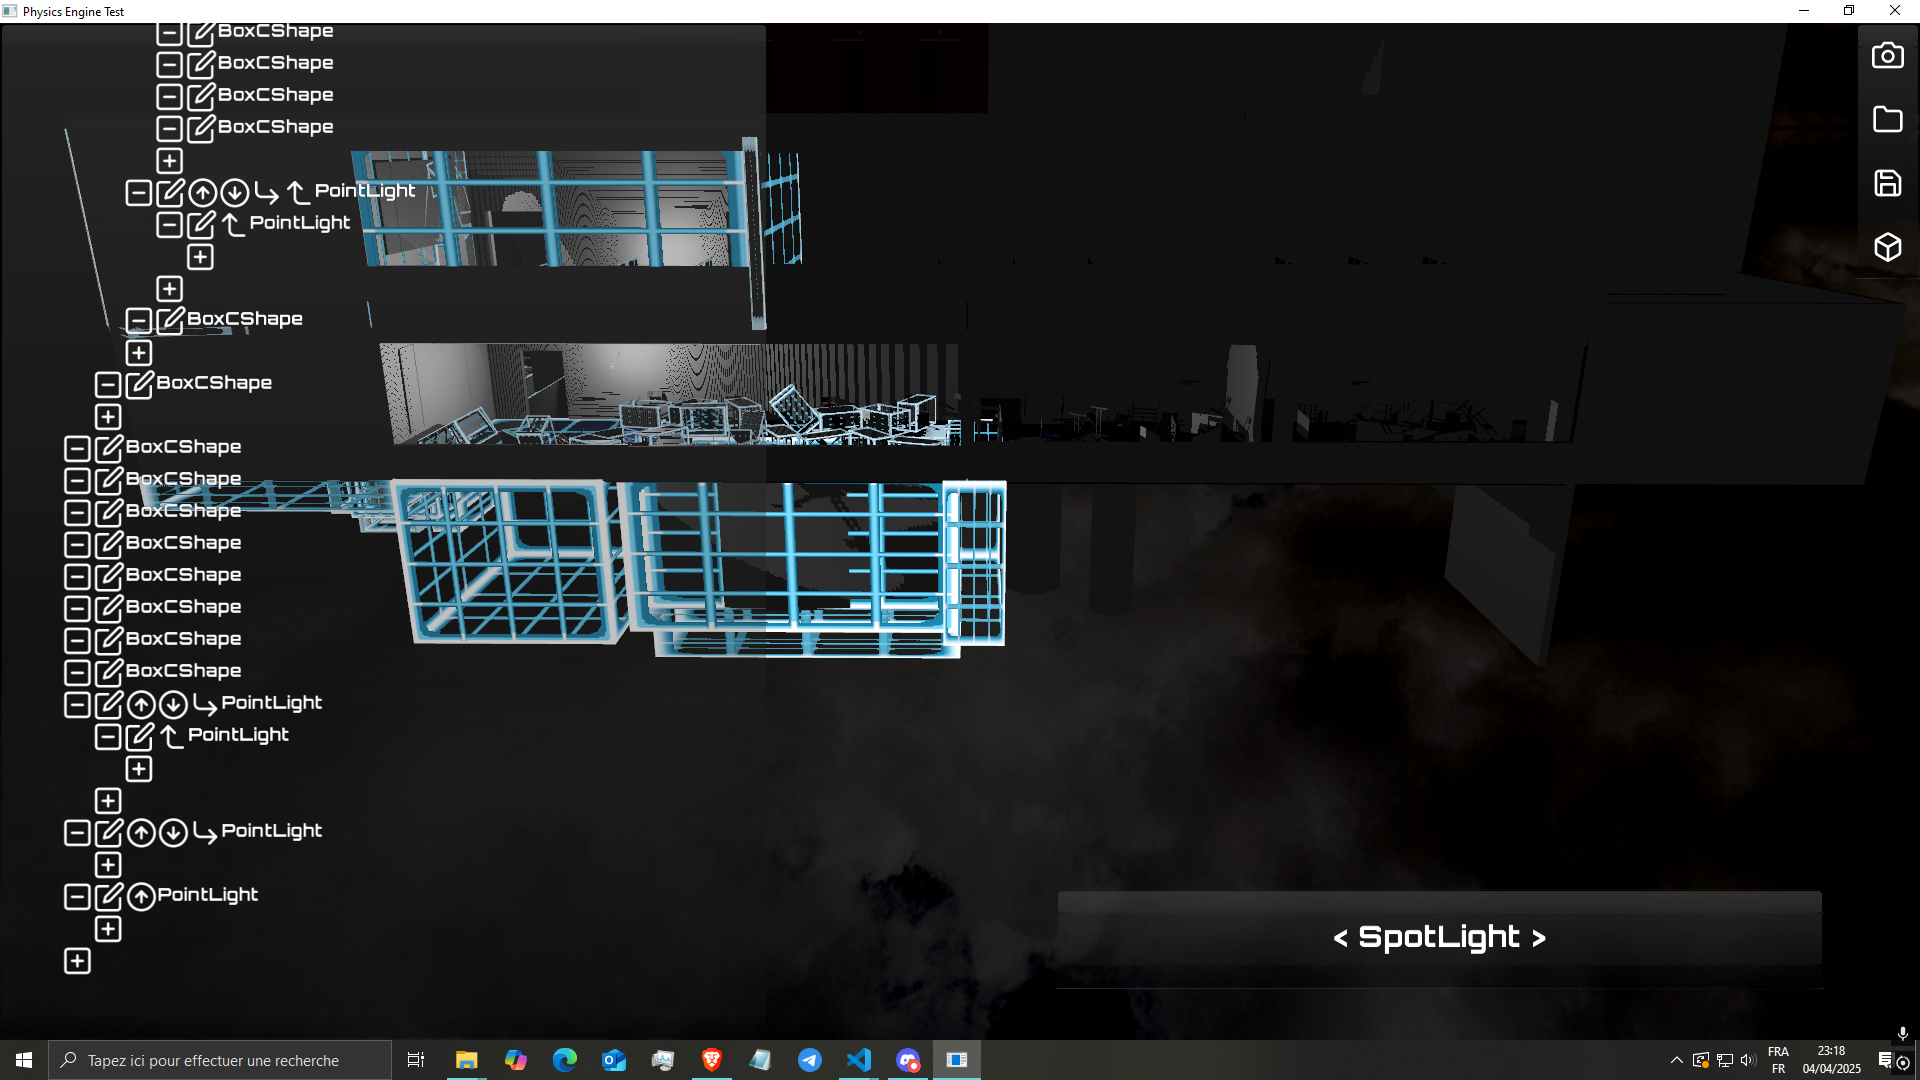
\includegraphics[width=0.8\textwidth]{images/gdb_editeur.png}
        \caption{Bug de collision}
        \label{fig:editeur1}
    \end{subfigure}
    \begin{subfigure}{0.5\textwidth}
        \centering
        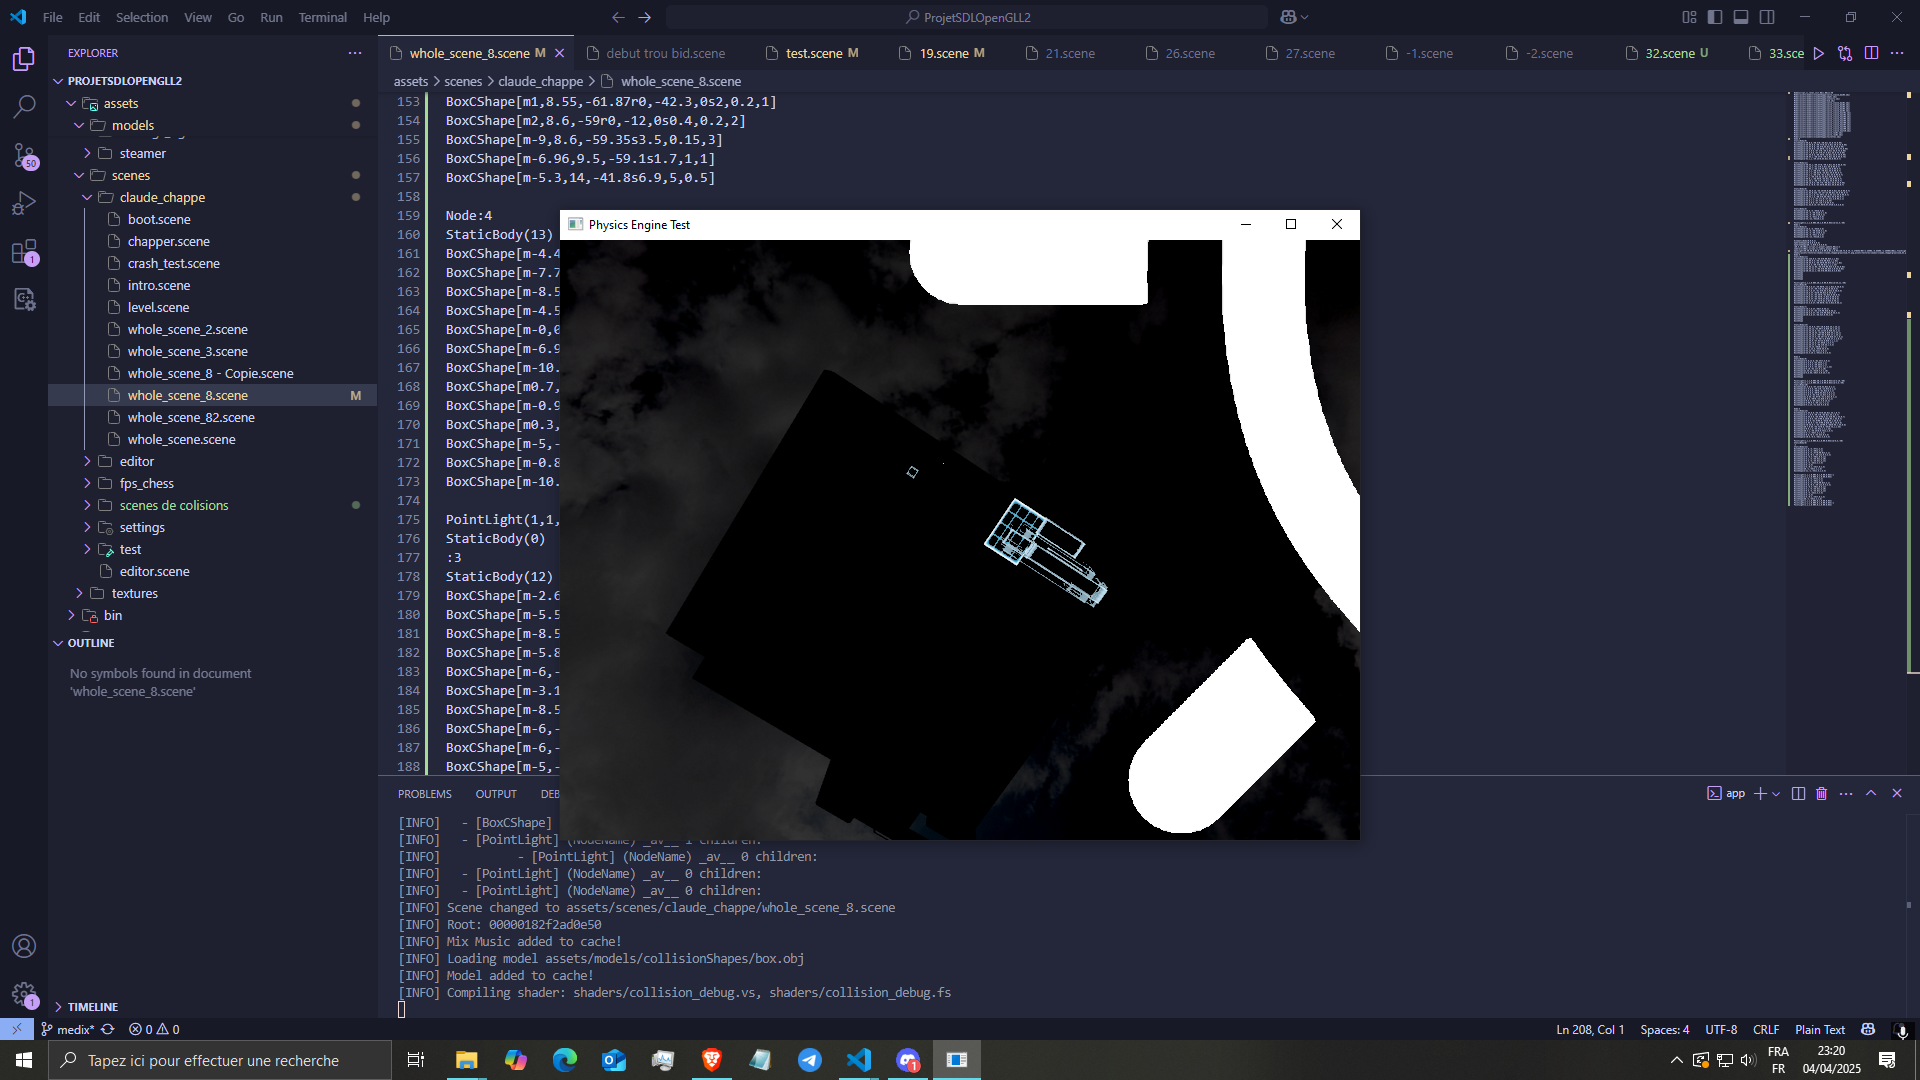
\includegraphics[width=0.8\textwidth]{images/gdb_editeur2.png}
        \caption{Bug de collision}
        \label{fig:editeur2}
    \end{subfigure}
    \begin{subfigure}{0.5\textwidth}
        \centering
        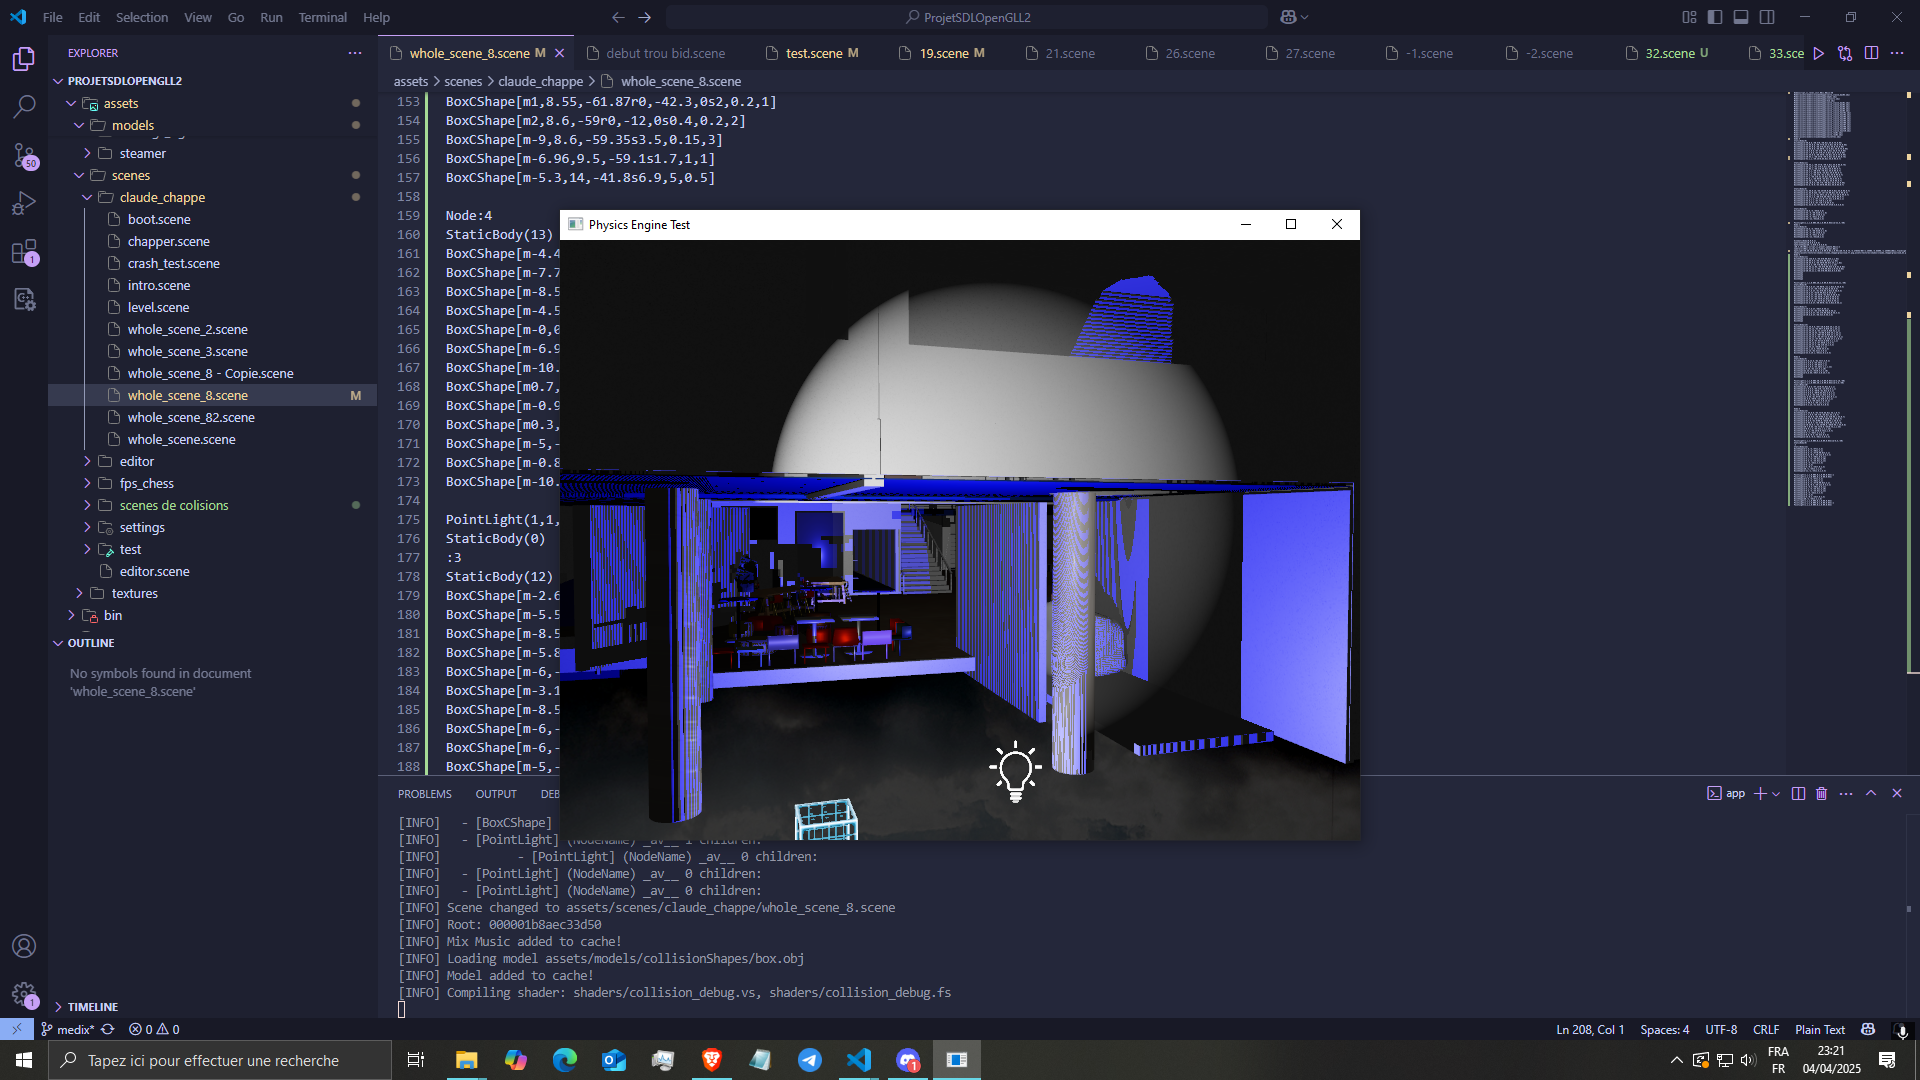
\includegraphics[width=0.8\textwidth]{images/gdb_editeur3.png}
        \caption{Bug d'affichage}
        \label{fig:editeur3}
    \end{subfigure}
    \caption{Exemples de bug à déboguer}
    \label{fig:debug}
\end{figure}

\begin{multicols}{2}
\begin{figure}[H]
    \centering
    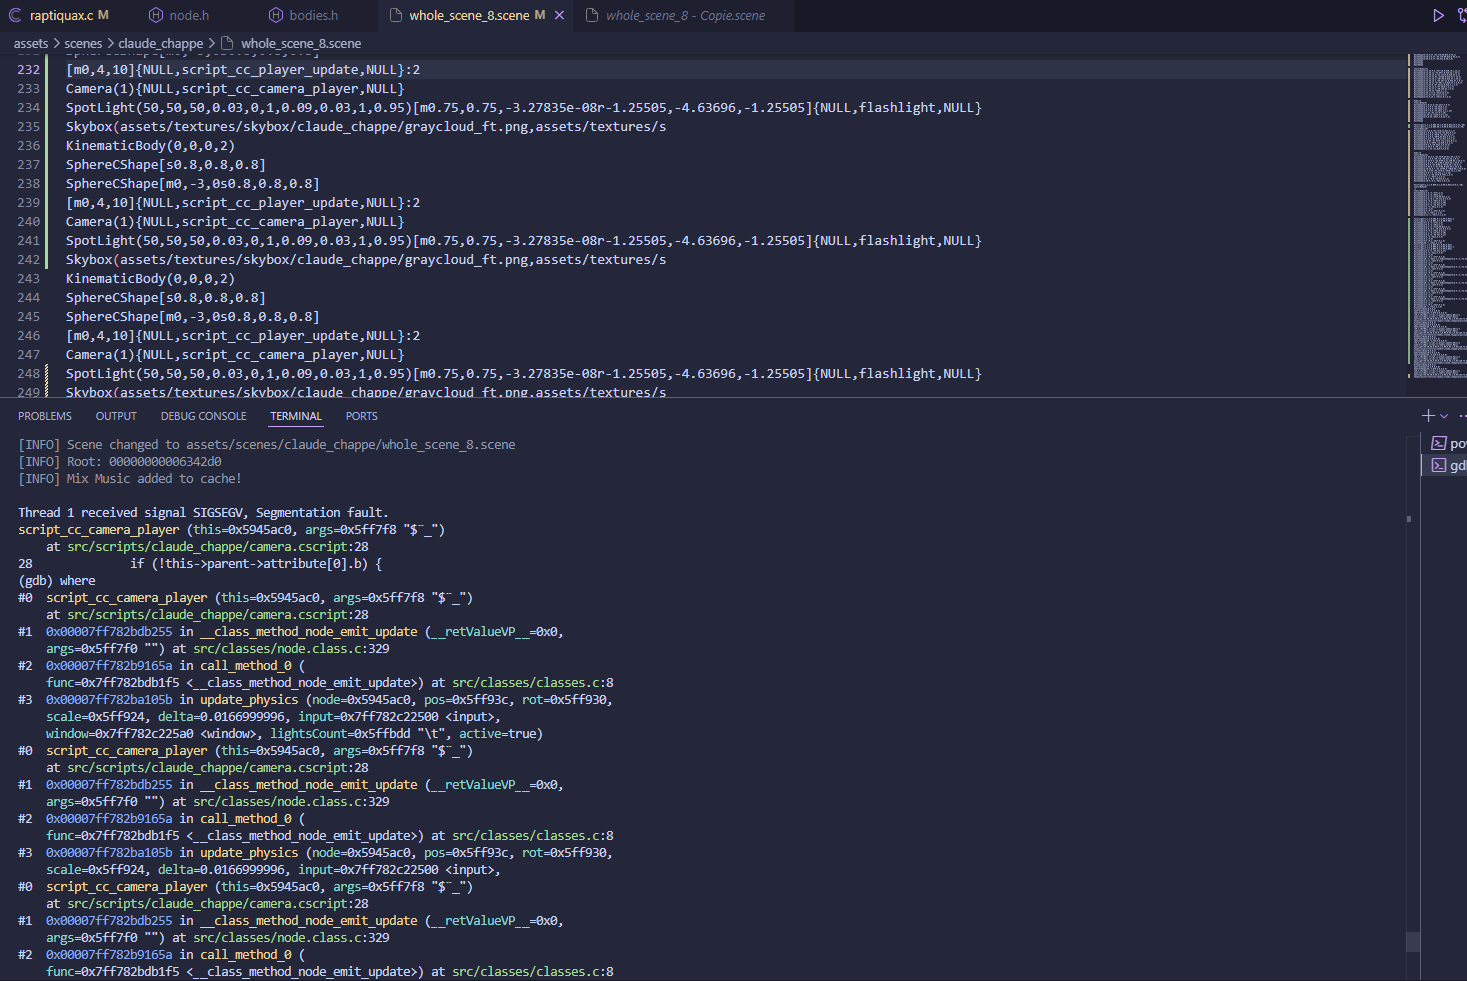
\includegraphics[width=0.5\textwidth]{images/gdb.png}
    \caption{Exemple de débogage avec GDB}
    \label{fig:debug}
\end{figure}

\begin{figure}[H]
    \centering
    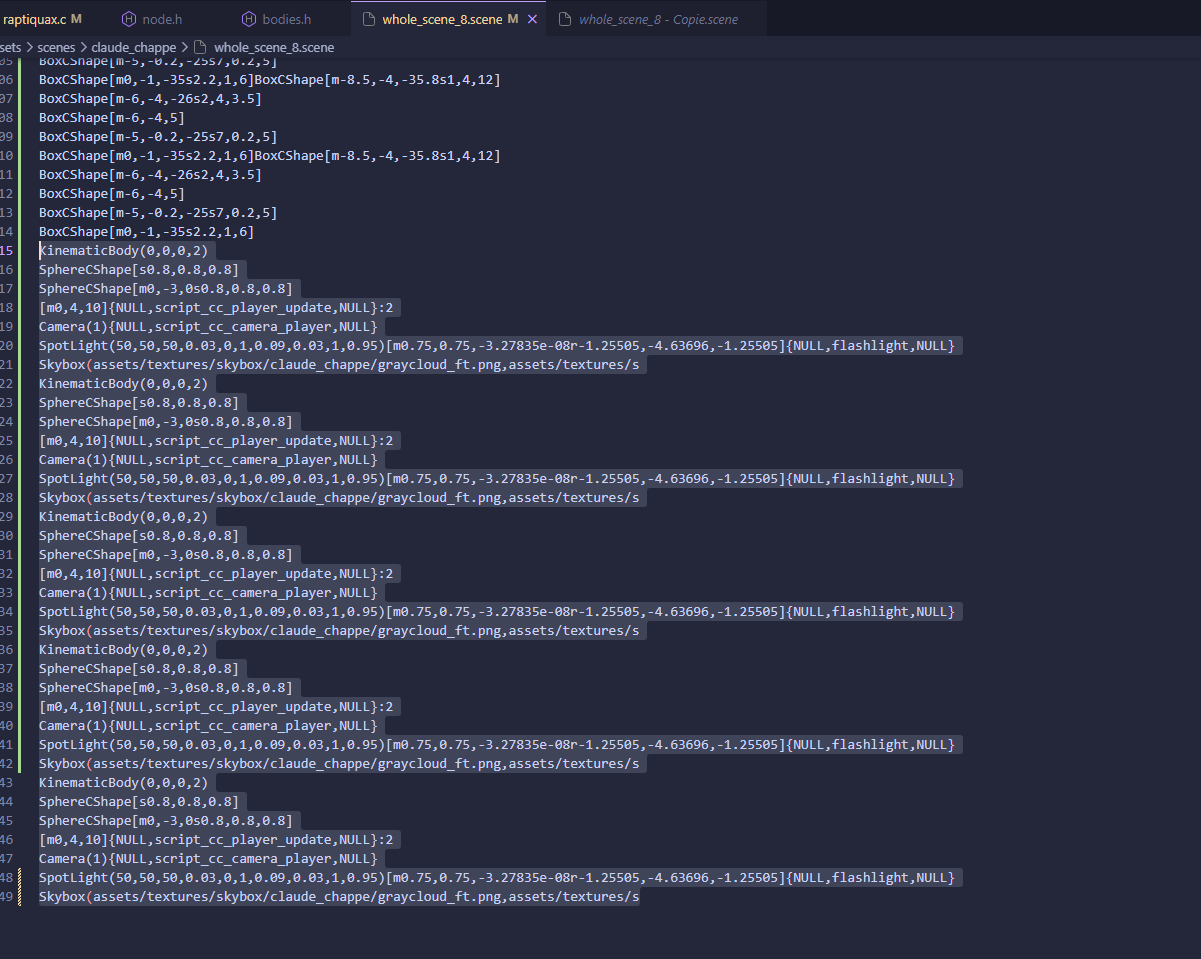
\includegraphics[width=0.5\textwidth]{images/gdb_fix.png}
    \caption{Correction du bug grâce à GDB}
    \label{fig:fix}
\end{figure}
\end{multicols}

\subsection{Code d'une classe générique}
\lstinputlisting[style=class_c,caption={Template de classe dans RaptiquaX},label=lst:class_template]{pages/developpement/class_templace.class.c}
\subsection{Rendu différé}
\label{sec:deferred_rendering}
Exemple de rendu différé :
\begin{figure}[h]
    \begin{subfigure}{0.5\textwidth}
        \centering
        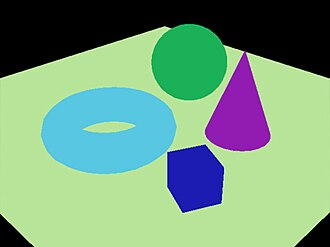
\includegraphics[width=0.8\textwidth]{images/Deferred_rendering_pass_col.jpg}
        \caption{G-Buffer de couleur}
        \label{fig:drendering_pass_col}
    \end{subfigure}
    \begin{subfigure}{0.5\textwidth}
        \centering
        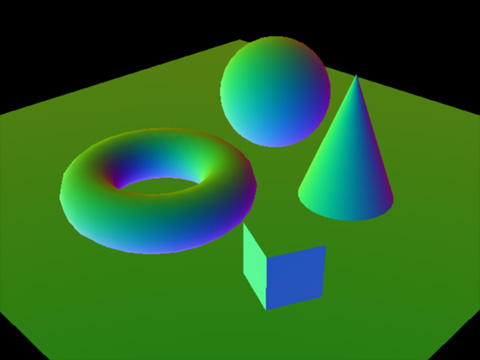
\includegraphics[width=0.8\textwidth]{images/Deferred_rendering_pass_nor.jpg}
        \caption{G-Buffer de normal}
        \label{fig:drendering_pass_normal}
    \end{subfigure}
    \begin{subfigure}{0.5\textwidth}
        \centering
        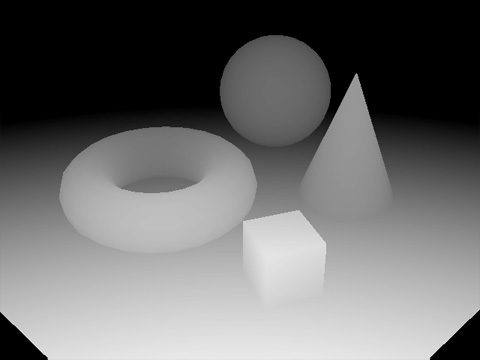
\includegraphics[width=0.8\textwidth]{images/Deferred_rendering_pass_dep.jpg}
        \caption{Z-Buffer}
        \label{fig:drendering_pass_depth}
    \end{subfigure}
    \begin{subfigure}{0.5\textwidth}
        \centering
        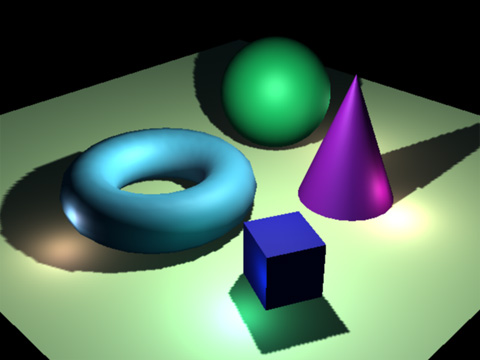
\includegraphics[width=0.8\textwidth]{images/Deferred_rendering_pass_res.jpg}
        \caption{Résultat final}
        \label{fig:drendering_result}
    \end{subfigure}
    \caption{Rendu différé d'une scène de volumes simples}
    \label{fig:defferred_rendering}
\end{figure}

\emph{Ici les Buffers ont été séparés pour montrer les différentes étapes du rendu différé.}

Le rendu différé s'appuie sur un G-Buffer qui contient les informations de la scène,
comme la couleur, les normaux et la profondeur. Ce G-Buffer est calculé en amont, lors
du rendu de la scène. C'est ensuite lors du rendu de la lumière et des effets de
post-processing qu'on utilise ce G-Buffer pour éviter de recalculer les informations de
la scène.
\newpage
\subsection{Pipeline graphique}
    \label{sec:graphics_pipeline}
    \begin{figure}[H]
        \begin{subfigure}{0.5\textwidth}
            \centering
            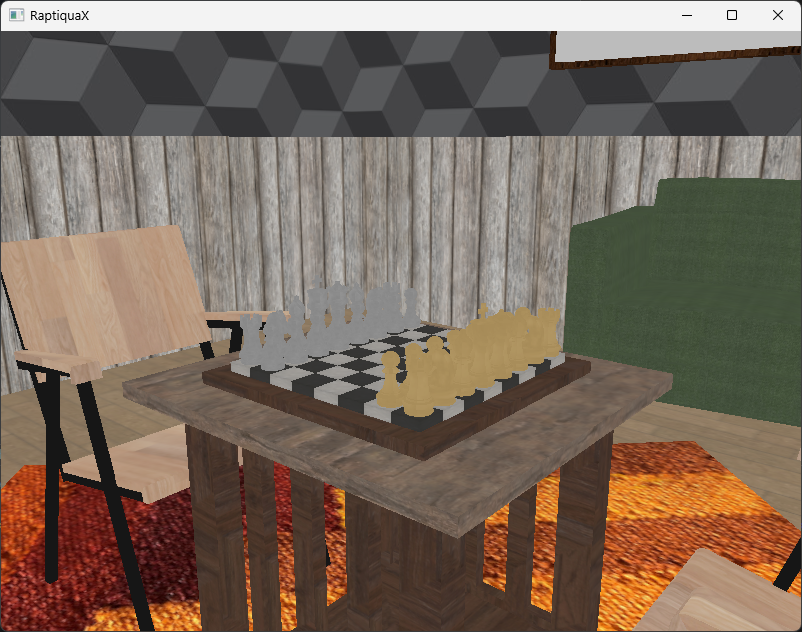
\includegraphics[width=0.8\textwidth]{images/raptiquax_rendering_gbuffer_albedo.png}
            \caption{G-Buffer de couleur}
            \label{fig:graphics_pipeline_gbuffer_albedo}
        \end{subfigure}
        \begin{subfigure}{0.5\textwidth}
            \centering
            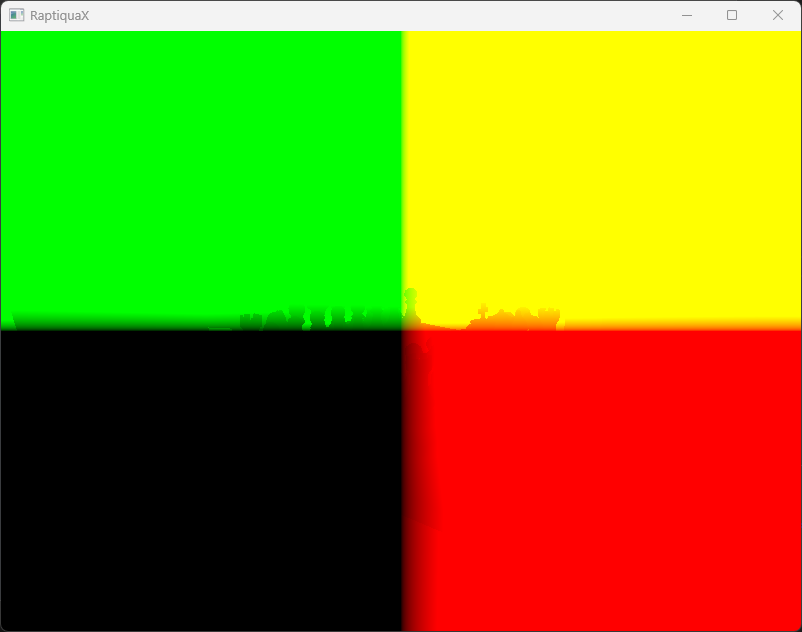
\includegraphics[width=0.8\textwidth]{images/raptiquax_rendering_gbuffer_position.png}
            \caption{G-Buffer de position}
            \label{fig:graphics_pipeline_gbuffer_position}
        \end{subfigure}
        \begin{subfigure}{0.5\textwidth}
            \centering
            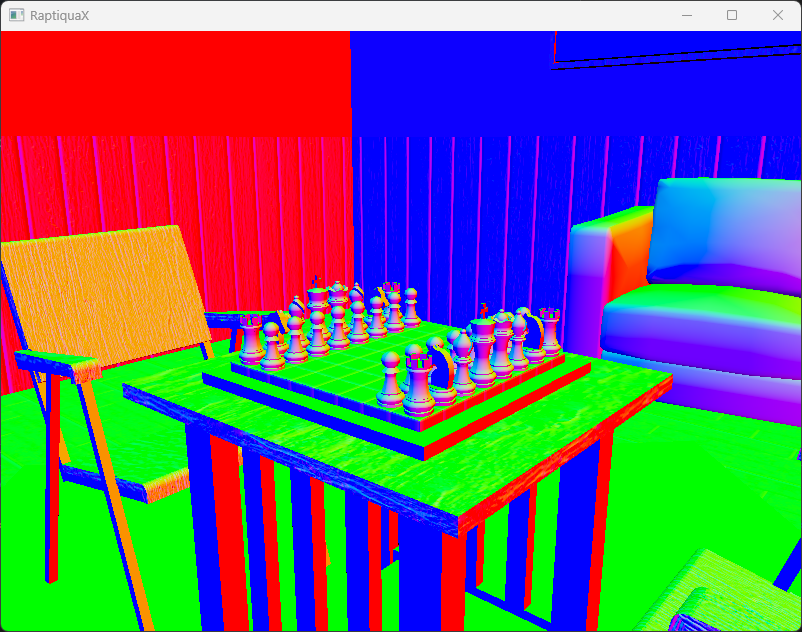
\includegraphics[width=0.8\textwidth]{images/raptiquax_rendering_gbuffer_normal.png}
            \caption{G-Buffer de normal}
            \label{fig:graphics_pipeline_gbuffer_normal}
        \end{subfigure}
        \begin{subfigure}{0.5\textwidth}
            \centering
            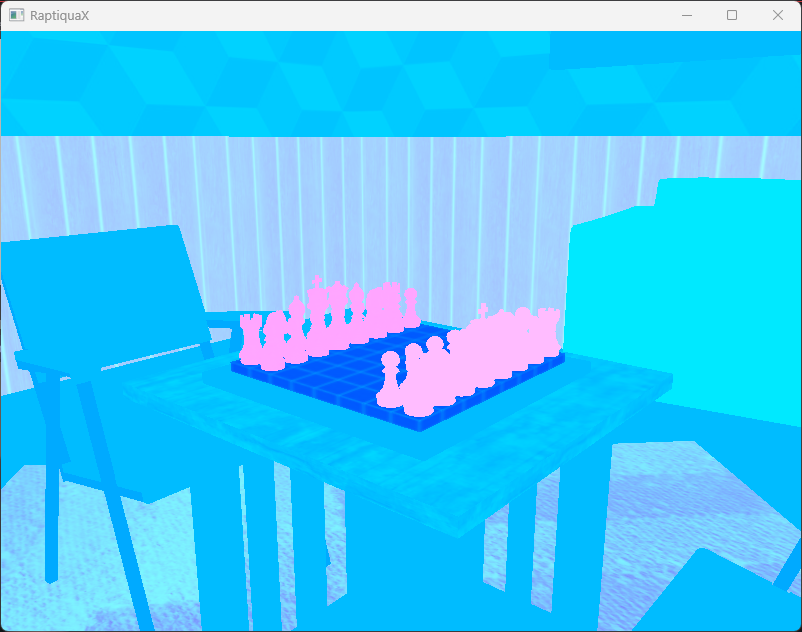
\includegraphics[width=0.8\textwidth]{images/raptiquax_rendering_gbuffer_extra.png}
            \caption{G-Buffer de métallicité et de rugosité}
            \label{fig:graphics_pipeline_gbuffer_color}
        \end{subfigure}
        \caption{G-Buffer de la scène}
        \label{fig:graphics_pipeline_gbuffer}
    \end{figure}
    \begin{figure}[H] 
        \begin{subfigure}{0.3\textwidth}
            \centering
            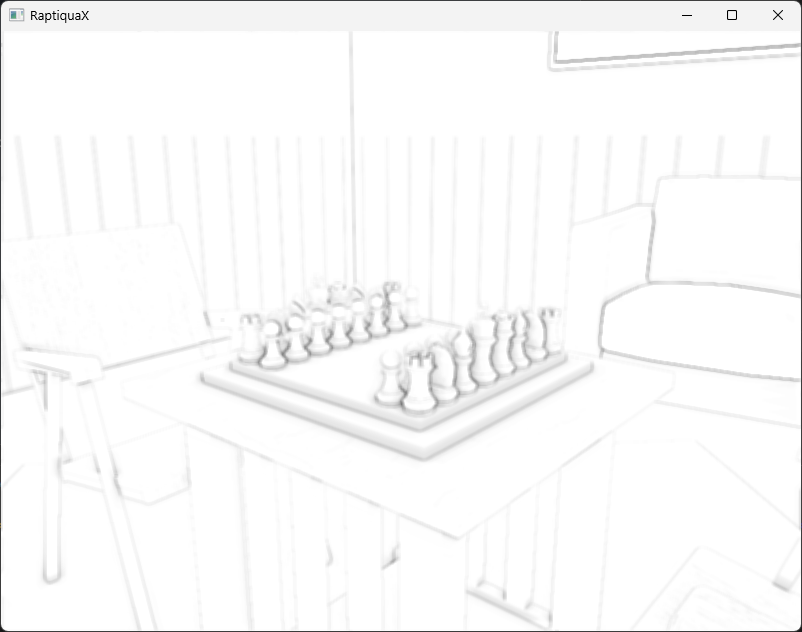
\includegraphics[width=0.8\textwidth]{images/raptiquax_rendering_ssao.png}
            \caption{Calque de l'occlusion ambiante}
            \label{fig:graphics_pipeline_gbuffer_ssao}
        \end{subfigure}
        \begin{subfigure}{0.3\textwidth}
            \centering
            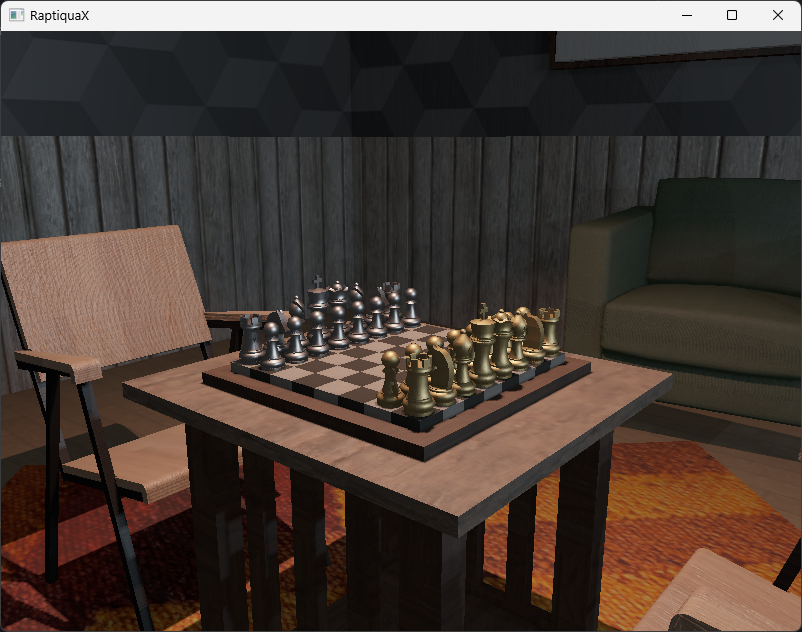
\includegraphics[width=0.8\textwidth]{images/raptiquax_rendering_lightings.png}
            \caption{Calque de la lumière et des ombres}
            \label{fig:graphics_pipeline_gbuffer_light}
        \end{subfigure}
        \begin{subfigure}{0.3\textwidth}
            \centering
            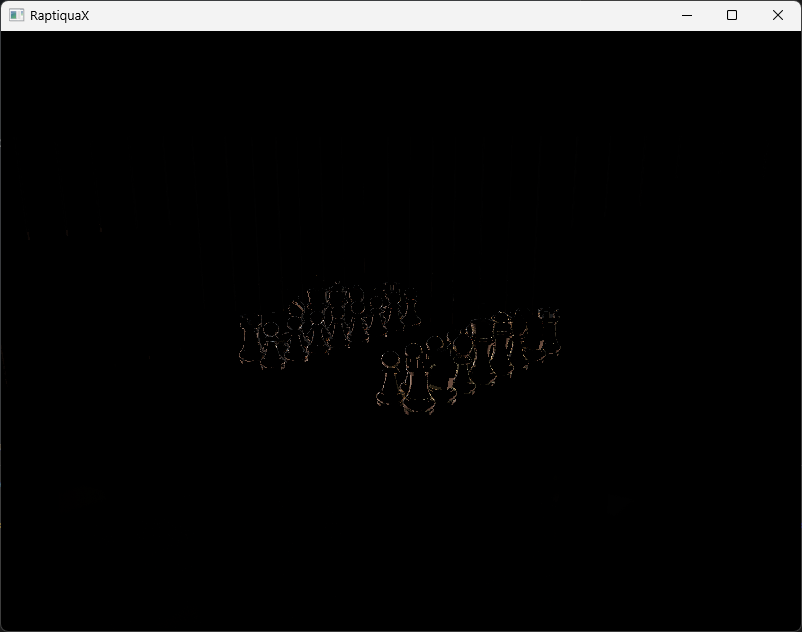
\includegraphics[width=0.8\textwidth]{images/raptiquax_rendering_ssr.png}
            \caption{Calque des réflexion et reflets}
            \label{fig:graphics_pipeline_gbuffer_ssr}
        \end{subfigure}
        \begin{subfigure}{0.3\textwidth}
            \centering
            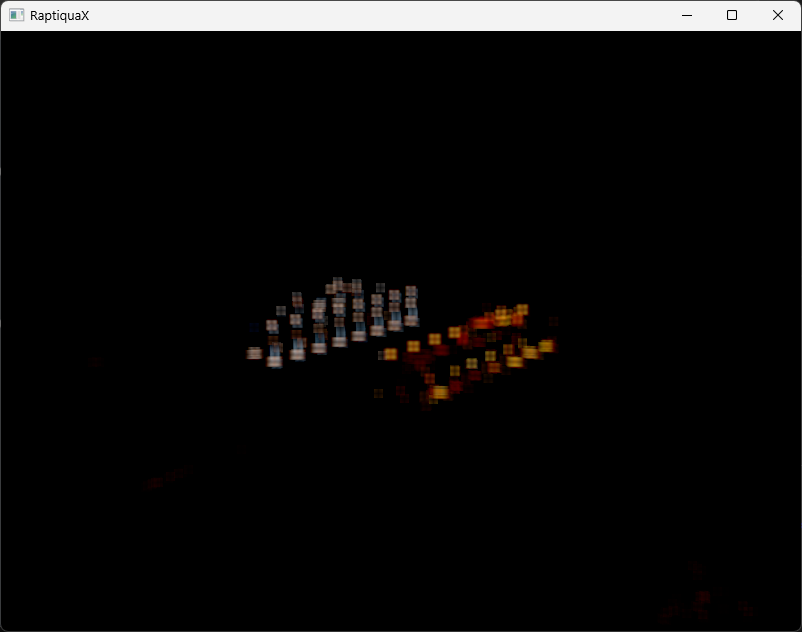
\includegraphics[width=0.8\textwidth]{images/raptiquax_rendering_bloom.png}
            \caption{Calque de l'éblouissement}
            \label{fig:graphics_pipeline_gbuffer_bloom}
        \end{subfigure}
        \begin{subfigure}{0.3\textwidth}
            \centering
            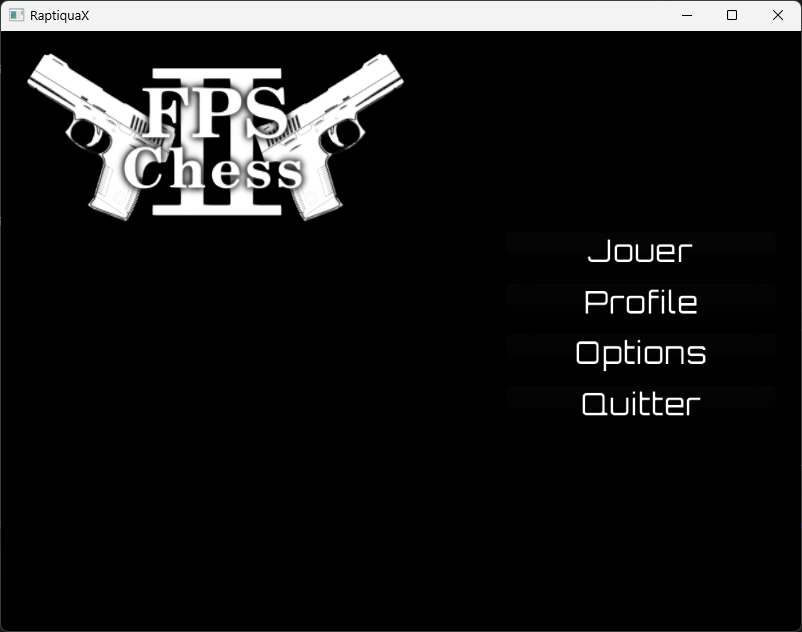
\includegraphics[width=0.8\textwidth]{images/raptiquax_rendering_gui.png}
            \caption{Calque de l'interface utilisateur}
            \label{fig:graphics_pipeline_gbuffer_gui}
        \end{subfigure}
        \caption{Calques de la scène}
        \label{fig:graphics_pipeline_post_processing}
    \end{figure}
    \begin{figure}[H]
        \centering
        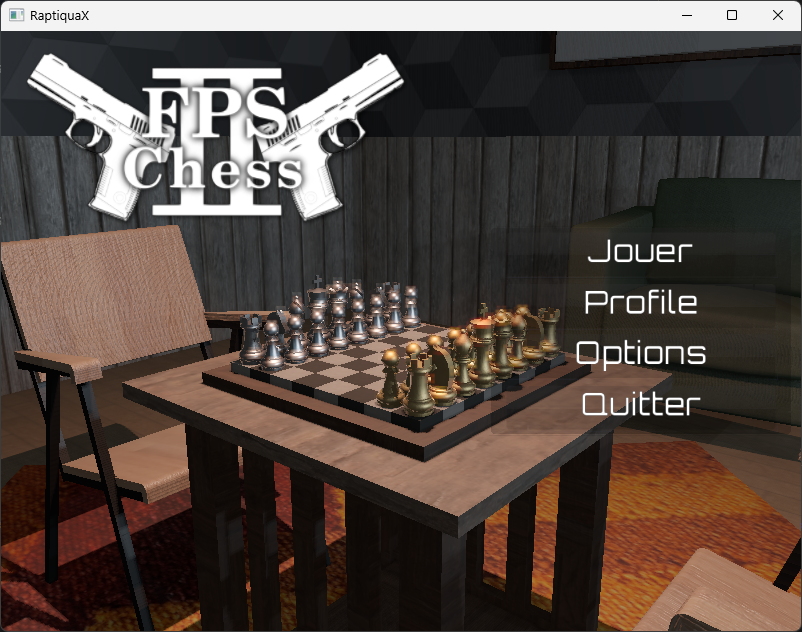
\includegraphics[width=0.5\textwidth]{images/raptiquax_rendering_result.png}
        \caption{Résultat de la pipeline graphique}
        \label{fig:graphics_pipeline_result}
    \end{figure}
\subsection{Musique}
\begin{figure}[H]
    \centering
    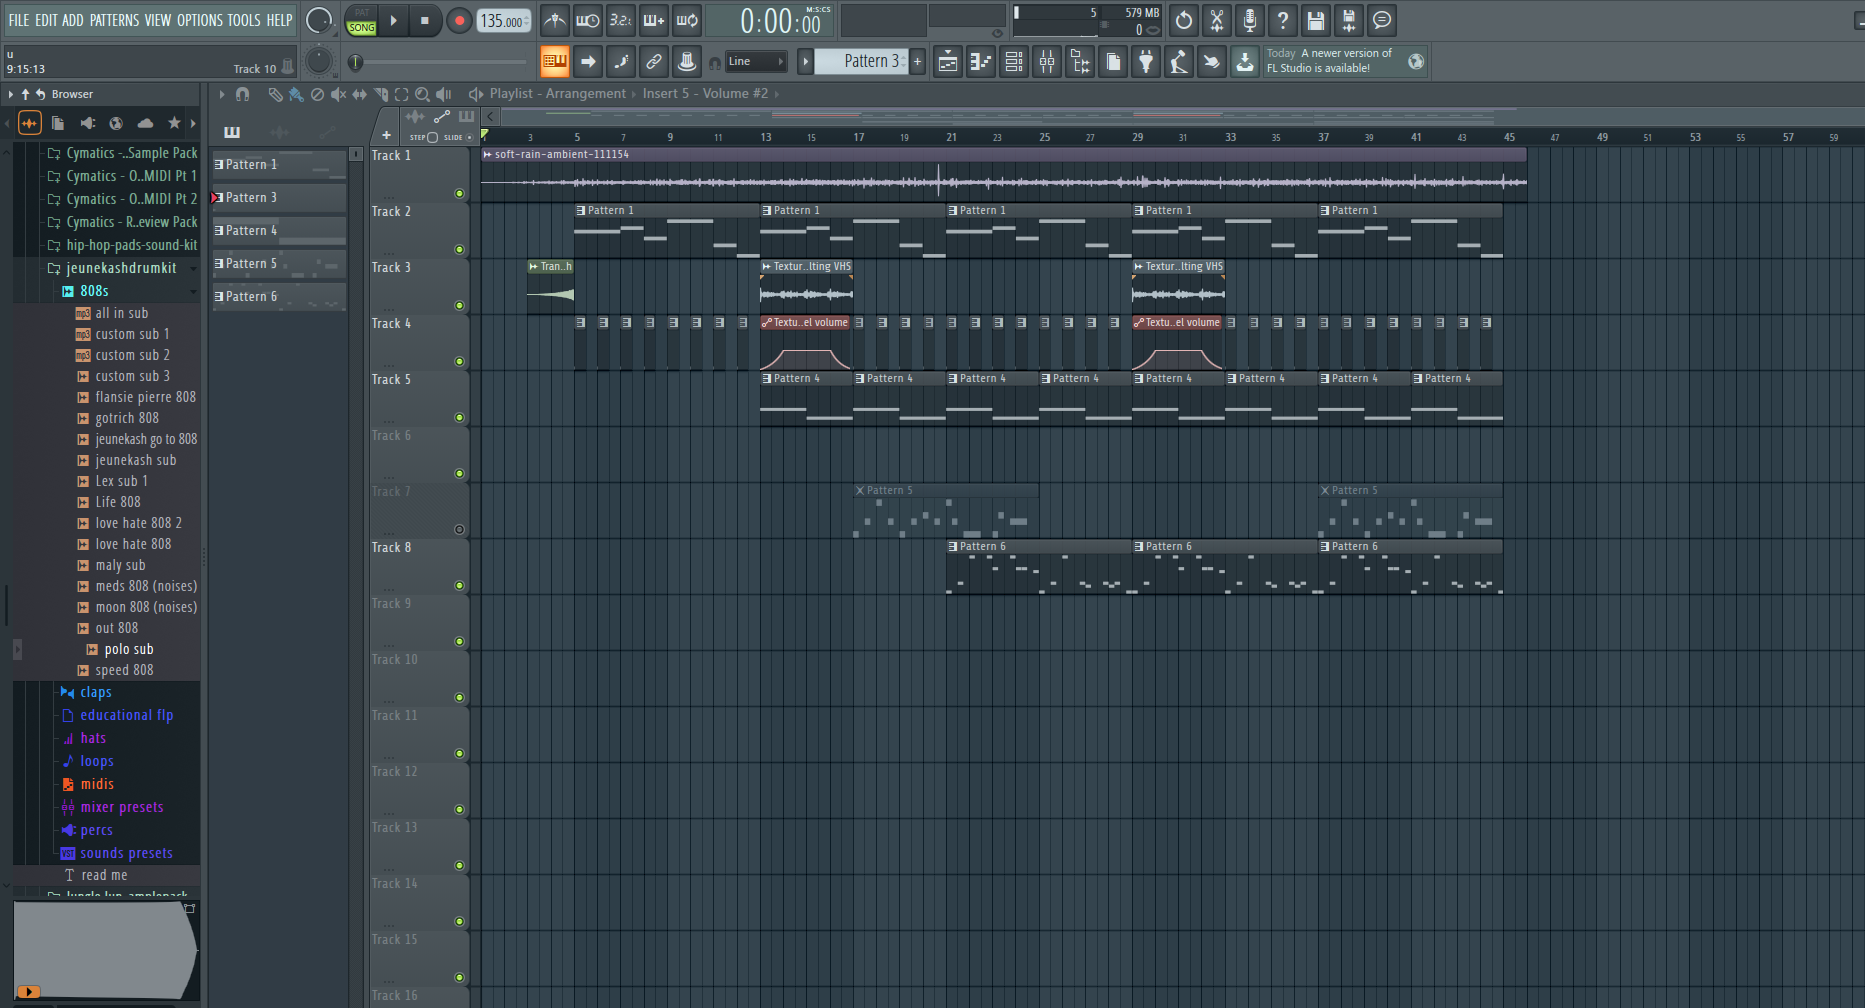
\includegraphics[width=1\linewidth]{images/flstudio.png}
    \caption{fl studio}
    \label{fig:flstudio.png}
\end{figure}

\newpage


\subsection{Équations de la physique}
    \label{sec:physics_equations}
    \paragraph{Norme de la collision}
    La norme de la collision entre les deux corps est donnée par un vecteur
    normal à la surface de collision. Si les corps ont une normale de
    collision définie, cette norme est utilisée dans les calculs suivants.

    \nomenclature{$\mathbf{n}$}{Vecteur normal à la surface de collision}
    \nomenclature{$\mathbf{\lambda}_A$}{Normale de l'objet $A$}
    \nomenclature{$\mathbf{\lambda}_B$}{Normale de l'objet $B$}

    \begin{equation}
    \mathbf{n} = \mathbf{\lambda}_A \cdot \mathbf{\lambda}_B
    \end{equation}

    \paragraph{Vitesse relative}
    La vitesse relative des deux objets rigides \( A \) et \( B \) est calculée
    comme la différence entre leurs vitesses respectives :

    \nomenclature{$\mathbf{v}_{\text{relative}}$}{Vitesse relative entre deux objets}
    \nomenclature{$\mathbf{v}_A$}{Vitesse de l'objet $A$}
    \nomenclature{$\mathbf{v}_B$}{Vitesse de l'objet $B$}

    \begin{equation}
    \mathbf{v}_{\text{relative}} = \mathbf{v}_B - \mathbf{v}_A
    \end{equation}

    \paragraph{Vitesse relative selon la direction normale}
    \nomenclature{$v_{\text{normal}}$}{Vitesse relative projetée sur la normale de collision}

    \begin{equation}
    v_{\text{normal}} = \mathbf{v}_{\text{relative}} \cdot \mathbf{n}
    \end{equation}

    \paragraph{Coefficient de restitution (élasticité de la collision)}
    \nomenclature{$e$}{Coefficient de restitution}

    \begin{equation}
    e = 0.02
    \end{equation}

    \paragraph{Calcul de l'impulsion}
    \nomenclature{$I_{scalaire}$}{Quantité scalaire représentant l'impulsion échangée}
    \nomenclature{$m_A$}{Masse de l'objet $A$}
    \nomenclature{$m_B$}{Masse de l'objet $B$}

    \begin{equation}
    I_{scalaire} = \frac{(1 + e) \cdot v_{\text{normal}}}{m_A^{-1} + m_B^{-1}}
    \end{equation}

    \paragraph{Calcul du vecteur d'impulsion}
    \nomenclature{$\mathbf{I}$}{Vecteur d'impulsion appliqué pendant la collision}

    \begin{equation}
    \mathbf{I} = I_{scalaire} \cdot \mathbf{n}
    \end{equation}

    \paragraph{Application de l'impulsion et du couple}
    \nomenclature{$\mathbf{r}_A$}{Vecteur du centre de masse de $A$ au point d’impact}
    \nomenclature{$\mathbf{r}_B$}{Vecteur du centre de masse de $B$ au point d’impact}
    \nomenclature{$\mathbf{C}_A$}{Centre de masse de $A$}
    \nomenclature{$\mathbf{C}_B$}{Centre de masse de $B$}
    \nomenclature{$\mathbf{P}_{\text{impact}}$}{Point d’impact}

    \begin{equation}
    \mathbf{r}_A = \mathbf{P}_{\text{impact}} - \mathbf{C}_A
    \end{equation}
    \begin{equation}
    \mathbf{r}_B = \mathbf{P}_{\text{impact}} - \mathbf{C}_B
    \end{equation}
    \begin{equation}
    \text{Couple sur A} = \mathbf{r}_A \times \mathbf{I}
    \end{equation}
    \begin{equation}
    \text{Couple sur B} = \mathbf{r}_B \times \mathbf{I}
    \end{equation}

    \paragraph{Application de l'impulsion}
    \nomenclature{$\mathbf{v}_A'$}{Nouvelle vitesse de l’objet $A$}
    \nomenclature{$\mathbf{v}_B'$}{Nouvelle vitesse de l’objet $B$}

    \begin{equation}
    \mathbf{v}_A' = \mathbf{v}_A + \mathbf{I} \cdot m_A^{-1}
    \end{equation}
    \begin{equation}
    \mathbf{v}_B' = \mathbf{v}_B - \mathbf{I} \cdot m_B^{-1}
    \end{equation}

    \paragraph{Correction de la pénétration}
    \nomenclature{$\delta$}{Profondeur de pénétration}
    \nomenclature{$\mathbf{C}$}{Correction appliquée pour compenser la pénétration}
    \nomenclature{$\mathbf{P}_A$}{Position initiale de l'objet $A$}
    \nomenclature{$\mathbf{P}_B$}{Position initiale de l'objet $B$}
    \nomenclature{$\mathbf{P}_A'$}{Nouvelle position de l'objet $A$}
    \nomenclature{$\mathbf{P}_B'$}{Nouvelle position de l'objet $B$}

    \[
    \mathbf{C} = \delta \cdot \mathbf{n}
    \]
    \begin{equation}
    \mathbf{P}_A' = \mathbf{P}_A - \mathbf{C}
    \end{equation}
    \begin{equation}
    \mathbf{P}_B' = \mathbf{P}_B + \mathbf{C}
    \end{equation}

    \paragraph{Calcul du couple et de l'inertie}
    \nomenclature{$\mathbf{I}_{\text{locale}}$}{Matrice d’inertie locale}
    \nomenclature{$w$}{Largeur de l'objet}
    \nomenclature{$h$}{Hauteur de l'objet}
    \nomenclature{$d$}{Profondeur de l'objet}

    \begin{equation}
    \mathbf{I}_{\text{locale}} = \frac{m}{12} \begin{bmatrix} h^2 + d^2 & 0 & 0 \\ 0 & w^2 + d^2 & 0 \\ 0 & 0 & w^2 + h^2 \end{bmatrix}
    \end{equation}

    \paragraph{Accélération angulaire}
    \nomenclature{$\mathbf{\alpha}$}{Accélération angulaire}
    \nomenclature{$\mathbf{T}$}{Couple appliqué}
    \nomenclature{$\mathbf{I}^{-1}$}{Inverse de la matrice d’inertie}

    \begin{equation}
    \mathbf{\alpha} = \mathbf{I}^{-1} \cdot \mathbf{T}
    \end{equation}

\subsection{Tableau des différents n\oe{}uds de la scène}
    \renewcommand{\arraystretch}{1.2}
    \setlength{\tabcolsep}{10pt}

    \begin{longtable}{>{\bfseries}p{0.25\linewidth} p{0.7\linewidth}}
        \toprule
        \textbf{Nœud} & \textbf{Description} \\
        \midrule
        Node & Classe de base pour tous les objets de la scène \\
        Camera & Représente un point de vue pour le rendu \\
        BoxCShape & Forme de collision en boîte \\
        CapsuleCShape & Forme de collision en capsule \\
        CShape & Classe de base des formes de collision \\
        MeshCShape & Forme de collision basée sur un maillage \\
        PlaneCShape & Plan infini utilisé pour les collisions \\
        RayCShape & Détecteur de collision basé sur un rayon \\
        SphereCShape & Forme de collision sphérique \\
        Button & Élément d'interface cliquable \\
        CheckBox & Case à cocher \\
        ControlFrame & Conteneur pour organiser l'interface \\
        Frame & Conteneur de base pour l'interface \\
        ImageFrame & Cadre affichant une image \\
        InputArea & Champ de saisie de texte \\
        Label & Étiquette de texte \\
        SelectList & Liste déroulante ou défilable \\
        Slider & Curseur pour sélectionner une valeur \\
        DirectionalLight & Source lumineuse directionnelle (\textit{ex : soleil}) \\
        Light & Classe de base pour les sources de lumière \\
        PointLight & Lumière omnidirectionnelle ponctuelle \\
        SpotLight & Source lumineuse en forme de cône \\
        Mesh & Maillage basique sans texture \\
        Model & Modèle 3D complet et texturé \\
        Area & Zone invisible déclenchant des événements \\
        Body & Classe de base pour les corps physiques \\
        KinematicBody & Corps physique contrôlé manuellement \\
        RigidBody & Objet physique entièrement simulé \\
        StaticBody & Corps physique immobile \\
        PhysicalNode & Base pour les nœuds liés à la physique \\
        RenderTarget & Sous scène rendu dans une texture \\
        Skybox & Cube d'environnement représentant le ciel \\
        TexturedMesh & Maillage avec textures appliquées \\
        \bottomrule
        \caption{Liste des n\oe{}uds de la scène}
        \label{tab:raptiquax_nodes}
    \end{longtable}

\subsection{Tableau des commandes Socket du mini-jeu \og FPS Chess \fg{}}
    \begin{table}[H]
        \centering
        \scriptsize
        \renewcommand{\arraystretch}{1.1}
        \begin{tabular}{|l|p{2.5cm}|p{4.5cm}|}
            \hline
            \textbf{Commande} & \textbf{Arguments} & \textbf{Description} \\
            \hline
            PONG & Aucun & Répond au ping du serveur. \\
            LOGIN & Nom d'utilisateur & Authentifie l'utilisateur et enregistre son nom. \\
            CREATE\_PARTY & Nom de la partie & Crée une nouvelle partie avec un nom donné. \\
            LIST\_PARTY & Aucun & Liste les parties existantes. \\
            EXIT\_PARTY & Aucun & Quitte la partie actuelle. \\
            JOIN\_PARTY & ID de la partie & Rejoint une partie donnée (par ID). \\
            RENAME\_PARTY & Nouveau nom & Renomme la partie actuelle. \\
            PARTY\_SET\_DATA & Clé=Valeur & Définit une valeur clé dans les données de la partie. \\
            PARTY\_GET\_DATA & Clé & Récupère une valeur clé des données de la partie. \\
            PARTY\_GET\_SELF\_INDEX & Aucun & Récupère l'index du joueur dans la partie. \\
            EXIT & Aucun & Déconnecte le client du serveur. \\
            G\_MSG & Message & Envoie un message global aux autres clients connectés. \\
            MSG & Message & Envoie un message à tous les joueurs de la partie ou globalement si hors partie. \\
            \hline
        \end{tabular}
        \caption{Requêtes gérées par le serveur SocketIO du moteur RaptiquaX}
        \label{tab:raptiquax_requests}
    \end{table}

\end{document}